\documentclass{beamer} 
\usepackage{amsmath,amsthm}
\usepackage{graphicx,microtype,parskip}
\usepackage{caption,subcaption,multirow}
\usepackage{attrib}

\frenchspacing

\usetheme{default}
\usecolortheme{whale}

\setbeamertemplate{navigation symbols}{}

\setbeamercolor{title}{fg=blue,bg=white}

\setbeamercolor{block title}{fg=white,bg=gray}
\setbeamercolor{block body}{fg=black,bg=lightgray}

\setbeamercolor{block title alerted}{fg=white,bg=darkgray}
\setbeamercolor{block body alerted}{fg=black,bg=lightgray}

\AtBeginSection[]
{
  \begin{frame}
    \tableofcontents[currentsection]
  \end{frame}
}


\title{Evolutionary paleoecology and \\the biology of extinction}
\author{Peter D Smits}
\institute{Committee on Evolutionary Biology, University of Chicago}

\begin{document}

\begin{frame}
  \begin{quotation}
    O species, stunned by your terror of chill death, why fear the Styx, why
    fear the ghosts and empty names, the stuff of poets, the spectres of a
    phantom world?

    \vspace{0.5cm}

    \tiny{\attrib{Ovid, \underline{Metamorphoses}, book XV: 143-–175, A. S. Kline trans.}}
  \end{quotation}
\end{frame}

\begin{frame}
  \maketitle
\end{frame}

\begin{frame}
  \tableofcontents
\end{frame}


\section{Theory}

\begin{frame}
  \frametitle{Extinction}

  \begin{quotation}
    All species that have ever lived are, to a first approximation, dead.

    \tiny{\attrib{Raup 1986 \underline{The Nemesis Affair}}}
  \end{quotation}
\end{frame}

\begin{frame}
  \frametitle{Foundation}

  \begin{alertblock}{Question}
    Why do certain taxa go extinct while others do not?
  \end{alertblock}
\end{frame}

\begin{frame}
  \frametitle{Modes of extinction}

  \hspace{\stretch{0.4}} Field of Bullets 
  \hspace{\stretch{0.5}} \textbf{--} 
  \hspace{\stretch{0.5}} Wanton 
  \hspace{\stretch{0.5}} \textbf{--} 
  \hspace{\stretch{0.5}} Fair Game 
  \hspace{\stretch{1}}

  \bigskip

  \tiny{\attrib{Raup 1991 \underline{Extinction: Bad Genes or Bad Luck?}}}

\end{frame}

\begin{frame}
  \frametitle{Evolutionary paleoecology}
  \begin{quotation}
    \dots the consequences of distinct ecological factors on differential rate dynamics, particularly rates of faunal turnover and diversification.

    \tiny{\attrib{Kitchell 1985 \textit{Paleobiology}}}
  \end{quotation}
\end{frame}

\begin{frame}
  \frametitle{In context of this study}

  \begin{block}{Rephrased}
    How does a taxon's \alert{adaptive zone} affect its \alert{extinction risk?}
  \end{block}
\end{frame}

\begin{frame}
  \frametitle{Adaptive zones}

  \begin{center}
    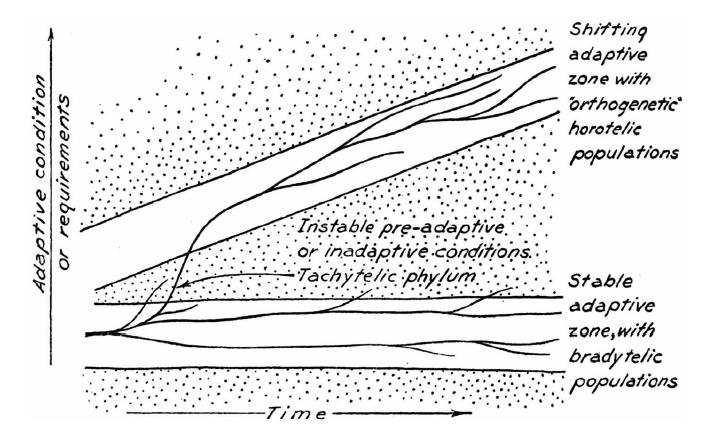
\includegraphics[height = 0.7\textheight, keepaspectratio = true]{figure/simpson}

    \tiny{\attrib{Simpson 1944 \underline{Tempo and Mode}}}
  \end{center}
\end{frame}

% Venn Diagram desbribing this
% would be easier to follow if came on piecewise
% avoid set building notation
\begin{frame}
  \frametitle{Simpson's terms}

  \begin{definition}
    \textbf{Environment:} The set of all possible interactions, both biotic and abiotic.
  
    \textbf{Adaptive zone:} The set of all interactions, biotic and abiotic, that a individual/taxon is adapted to or experiences in a given environment.
  \end{definition}

  \tiny{\attrib{Simpson 1944 \underline{Tempo and Mode}, Simpson 1953 \underline{Major Features}}}

\end{frame}

\begin{frame}
  \frametitle{Van Valen's observation}

  \begin{center}
    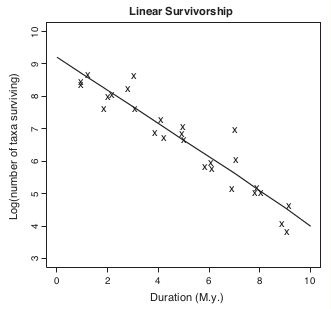
\includegraphics[height = 0.7\textheight, keepaspectratio = true]{figure/liow}

    \tiny{\attrib{Liow et al. 2011 \textit{TREE}}}
  \end{center}
\end{frame}

\begin{frame}
  \frametitle{Theory}

  \begin{alertblock}{Law of Constant Extinction}
    Extinction risk, in a given adaptive zone, is taxon--age independent.
  \end{alertblock}

  \tiny{\attrib{Van Valen 1973 \textit{Evol. Theory}}}

\end{frame}

\begin{frame}
  \frametitle{Approach}

  \begin{block}{Analytical challenge}
    Model extinction in context of adaptive zone (\alert{selective pressures}).
  \end{block}

  \vspace{1cm}

  \begin{columns}
    \begin{column}{0.5\textwidth}
      Survival
      \begin{itemize}
        \item traits, factors and duration
        \item extinction mode
      \end{itemize}
    \end{column}
    \begin{column}{0.5\textwidth}
      Communities
      \begin{itemize}
        \item \(\alpha, \beta\) diversity
        \item biome distinctiveness
      \end{itemize}
    \end{column}
  \end{columns}

\end{frame}

\begin{frame}
  \frametitle{Systems}

  \begin{columns}
    \begin{column}{0.5\textwidth}
      \begin{center}
        \textbf{Brachiopods}

        \vspace{0.5cm}

        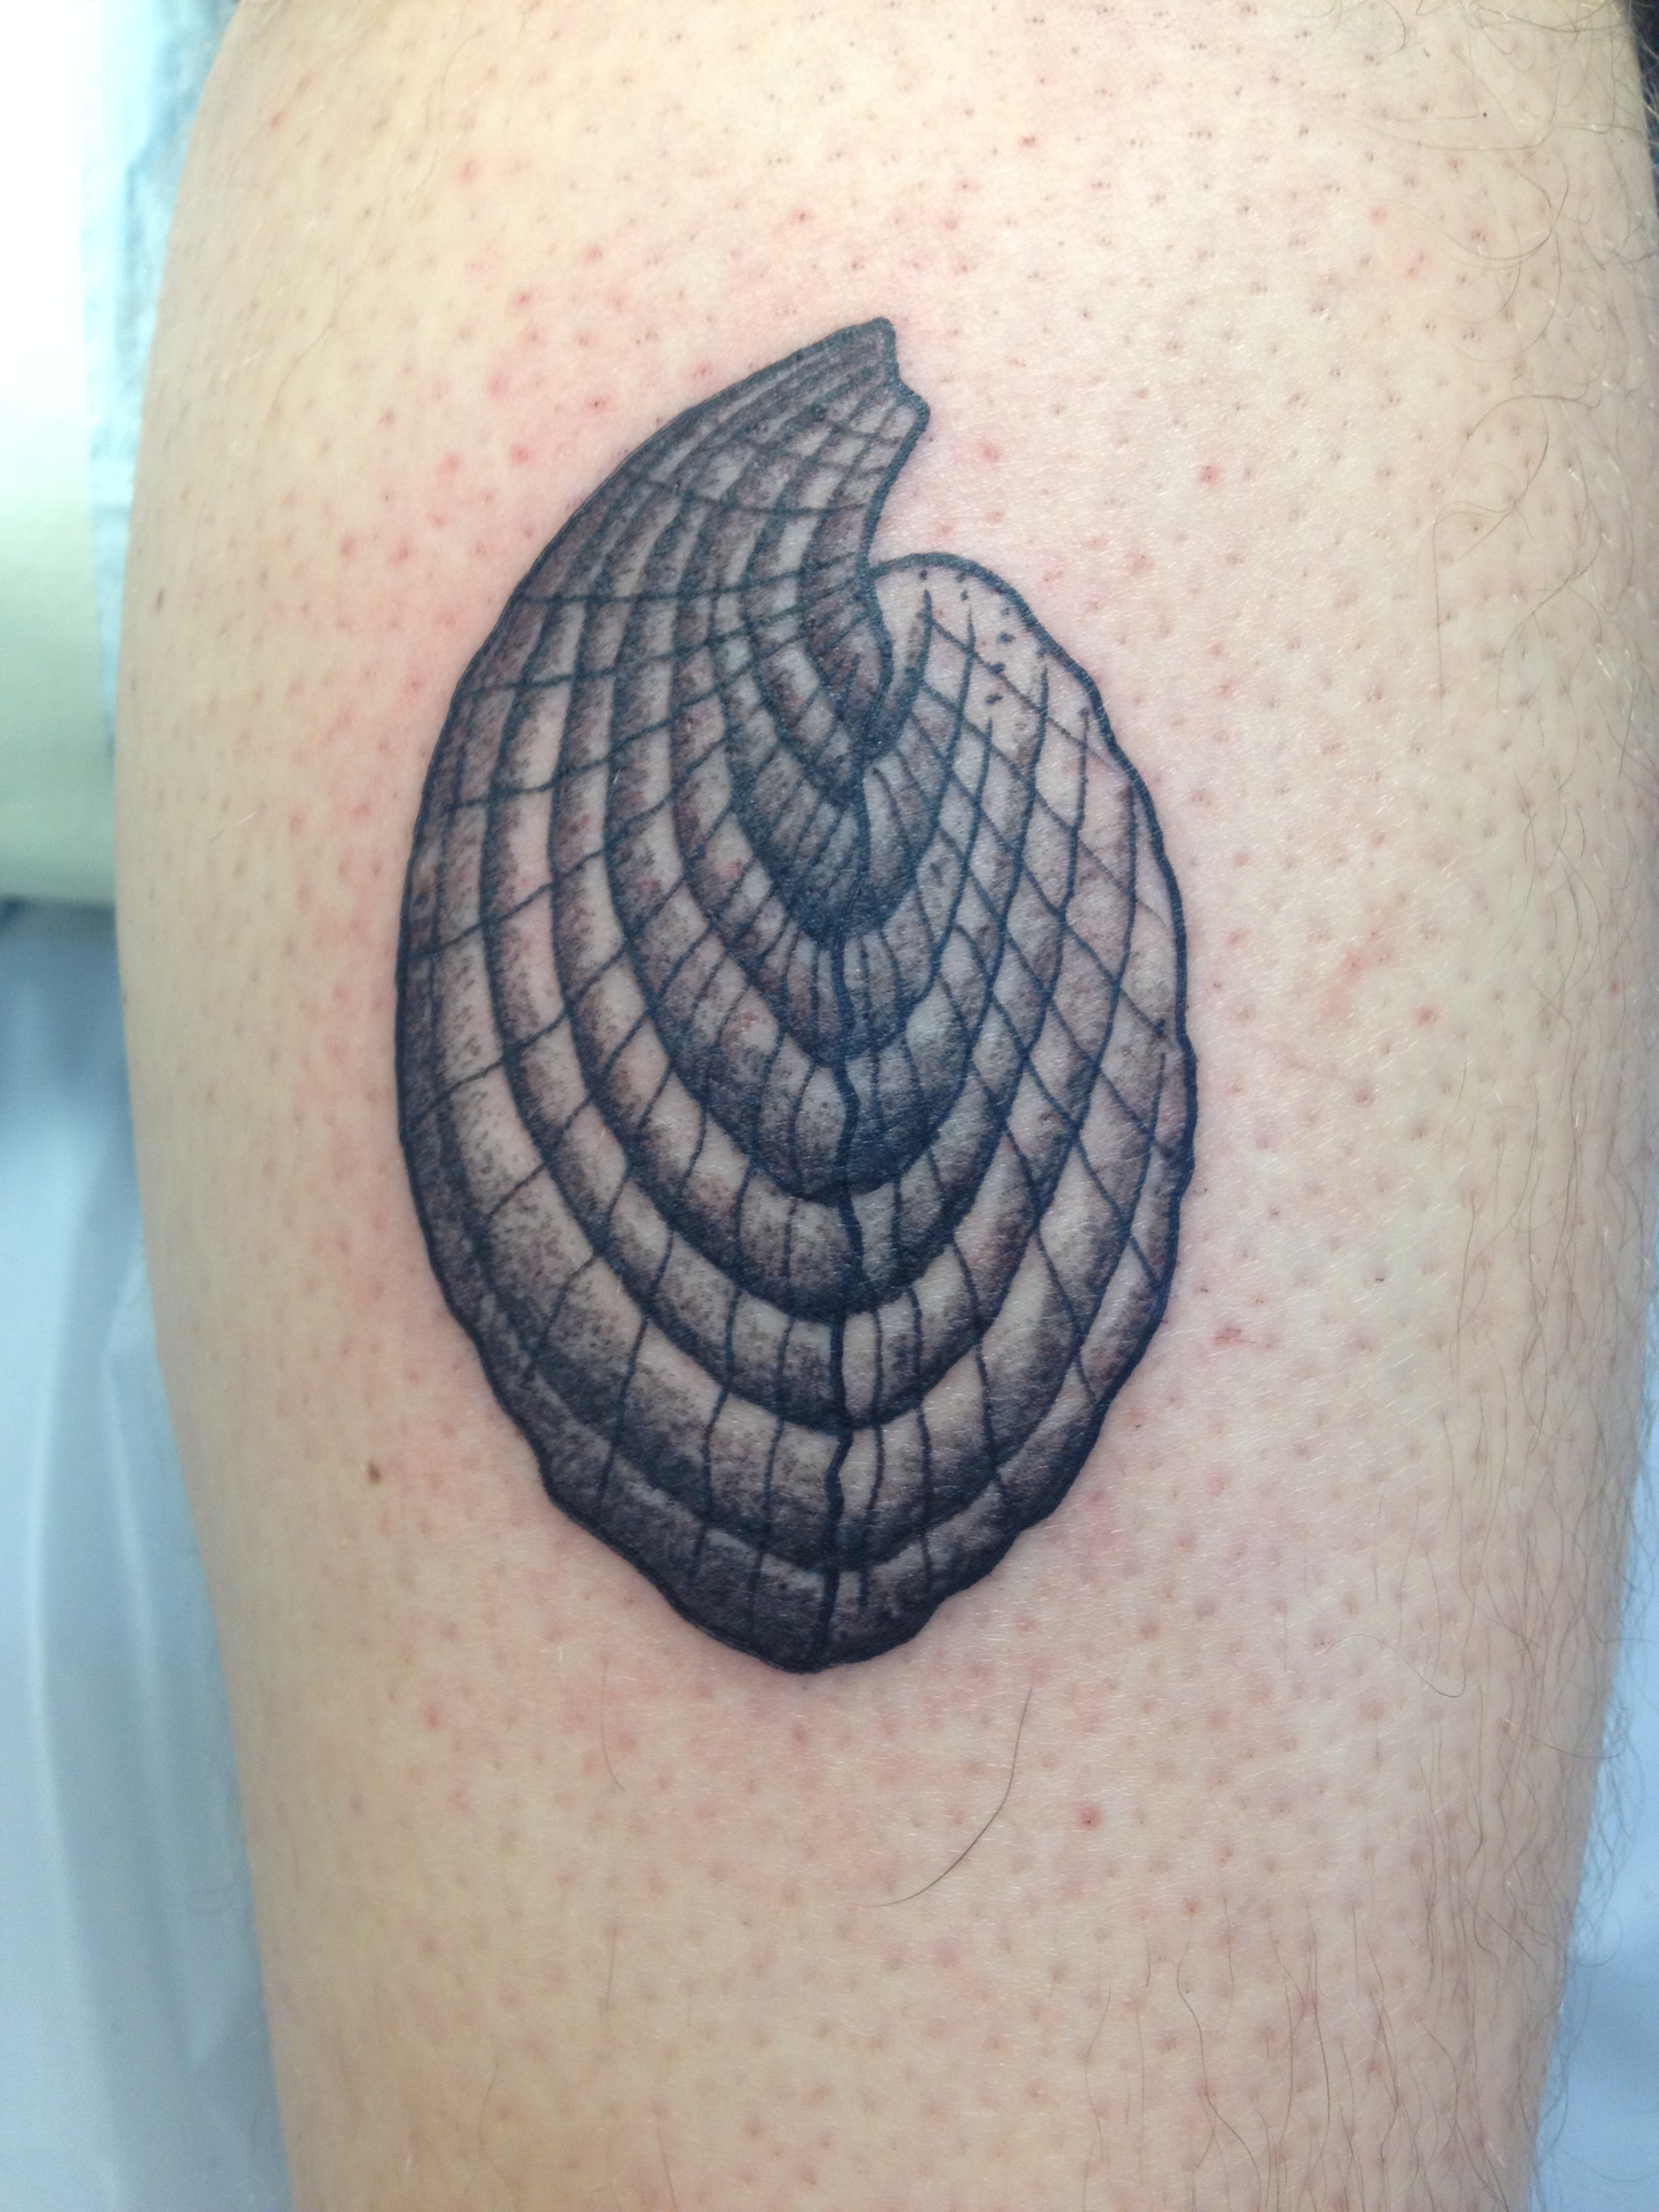
\includegraphics[height = 0.4\textheight, keepaspectratio = true]{figure/tattoo}
      \end{center}
    \end{column}
    \begin{column}{0.5\textwidth}
      \begin{center}
        \textbf{Mammals}

        \vspace{0.5cm}

        
\includegraphics[height = 0.4\textheight, keepaspectratio = true]{figure/annyong}
      \end{center}
    \end{column}
  \end{columns}
\end{frame}

\begin{frame}
  \frametitle{Proposed studies}

  Australian Permian brachiopods
  \begin{itemize}
    \item survival patterns
    \item community connectedness (not shown)
    \item substrate, habitat, affixing strategy
  \end{itemize}

  \vspace{1cm}

  Cenozoic mammals
  \begin{itemize}
    \item survival patterns (not shown; come to Evolution2014)
    \item community connectedness
    \item dietary and locomotor categories, body size
  \end{itemize}

\end{frame}


\section{Survival}

\begin{frame}
  \frametitle{Survival}

  \begin{definition}
    Time from origination to extintion of a taxon (age).
  \end{definition}

\end{frame}

\begin{frame}
  \frametitle{Brachiopods}
  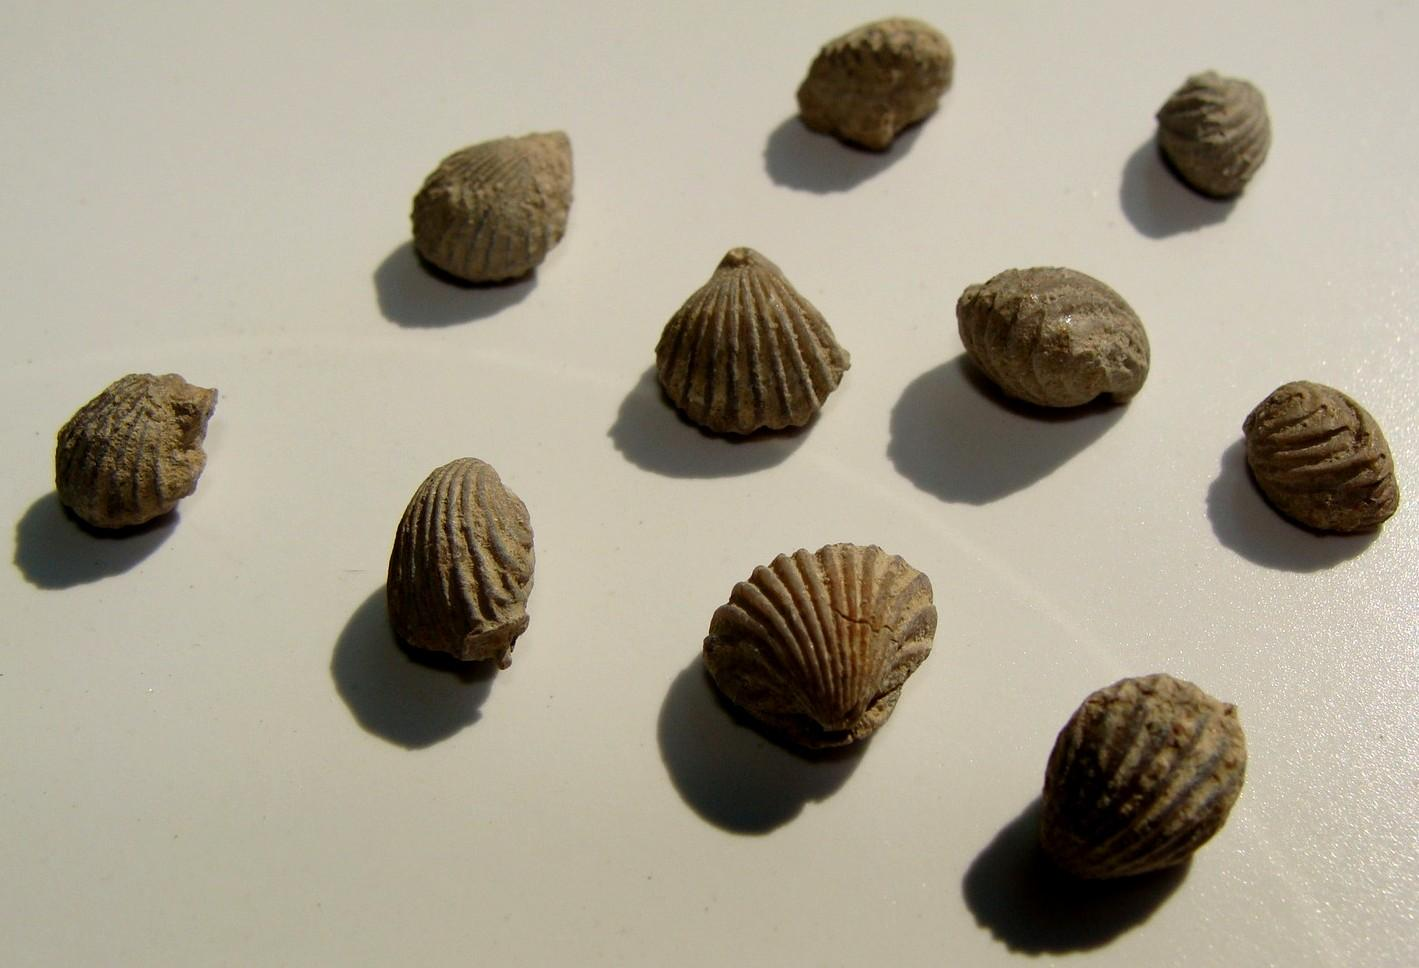
\includegraphics[height = 0.9\textheight, width = \textwidth, keepaspectratio = true]{figure/permian_brac}

  \tiny{\attrib{\url{http://earthphysicsteaching.homestead.com}}}
\end{frame}

\begin{frame}
  \frametitle{Permian}
  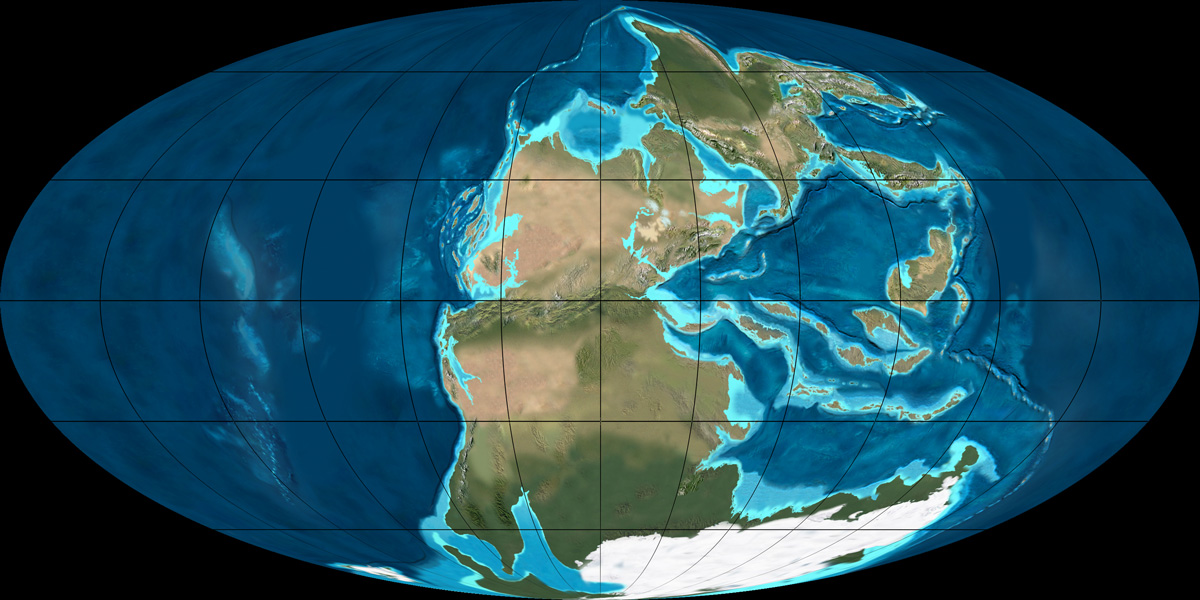
\includegraphics[height = \textheight, width = \textwidth, keepaspectratio = true]{figure/per_map}

  \tiny{\attrib{Blakey \url{http://cpgeosystems.com/mollglobe.html}}}
\end{frame}

\begin{frame}
  \frametitle{Permian of Australia}
  \begin{center}
    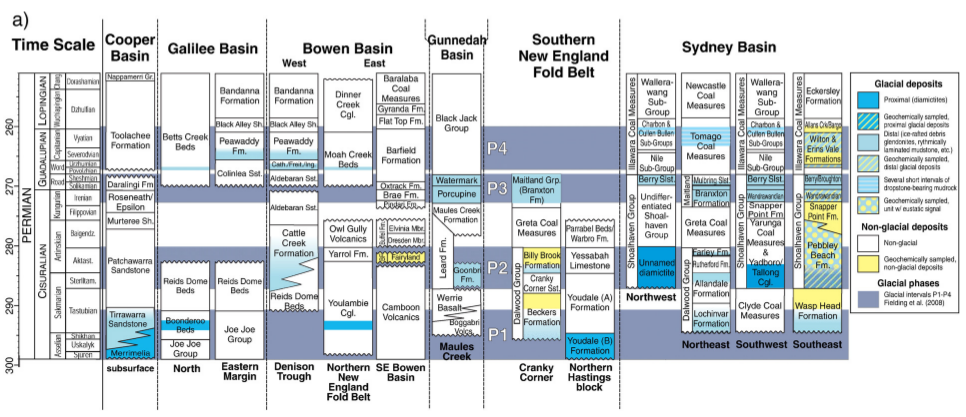
\includegraphics[height = 0.8\textheight, width = \textwidth, keepaspectratio = true]{figure/glacial}

    \tiny{\attrib{Birgenheier \textit{et al.} 2010 \textit{Paleo\(^3\)}}}
  \end{center}
\end{frame}

\begin{frame}
  \frametitle{Brachiopods, environmental preference, and extinction}

  \begin{block}{Questions}
    \begin{itemize}
      \item Do interactions involved in environmental preference predict differential survival?
        \begin{itemize}
          \item Is survival best modeled by a single interactor or multiple interactors? 
          \item How do other factors, such as climate, contribute?
        \end{itemize}
      \item Is extinction taxon-age independent or dependent?
    \end{itemize}
  \end{block}
\end{frame}

\begin{frame}
  \frametitle{Probability of survival}
  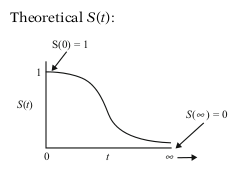
\includegraphics[height = 0.4\textheight, width = \textwidth, keepaspectratio = true]{figure/ideal}
  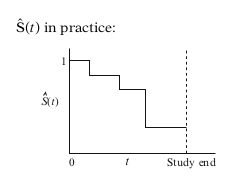
\includegraphics[height = 0.4\textheight, width = \textwidth, keepaspectratio = true]{figure/prac}

  \tiny{\attrib{Kleinbaum and Klein 2012}}
\end{frame}

\begin{frame}
  \frametitle{Extinction function}

  \begin{center}
    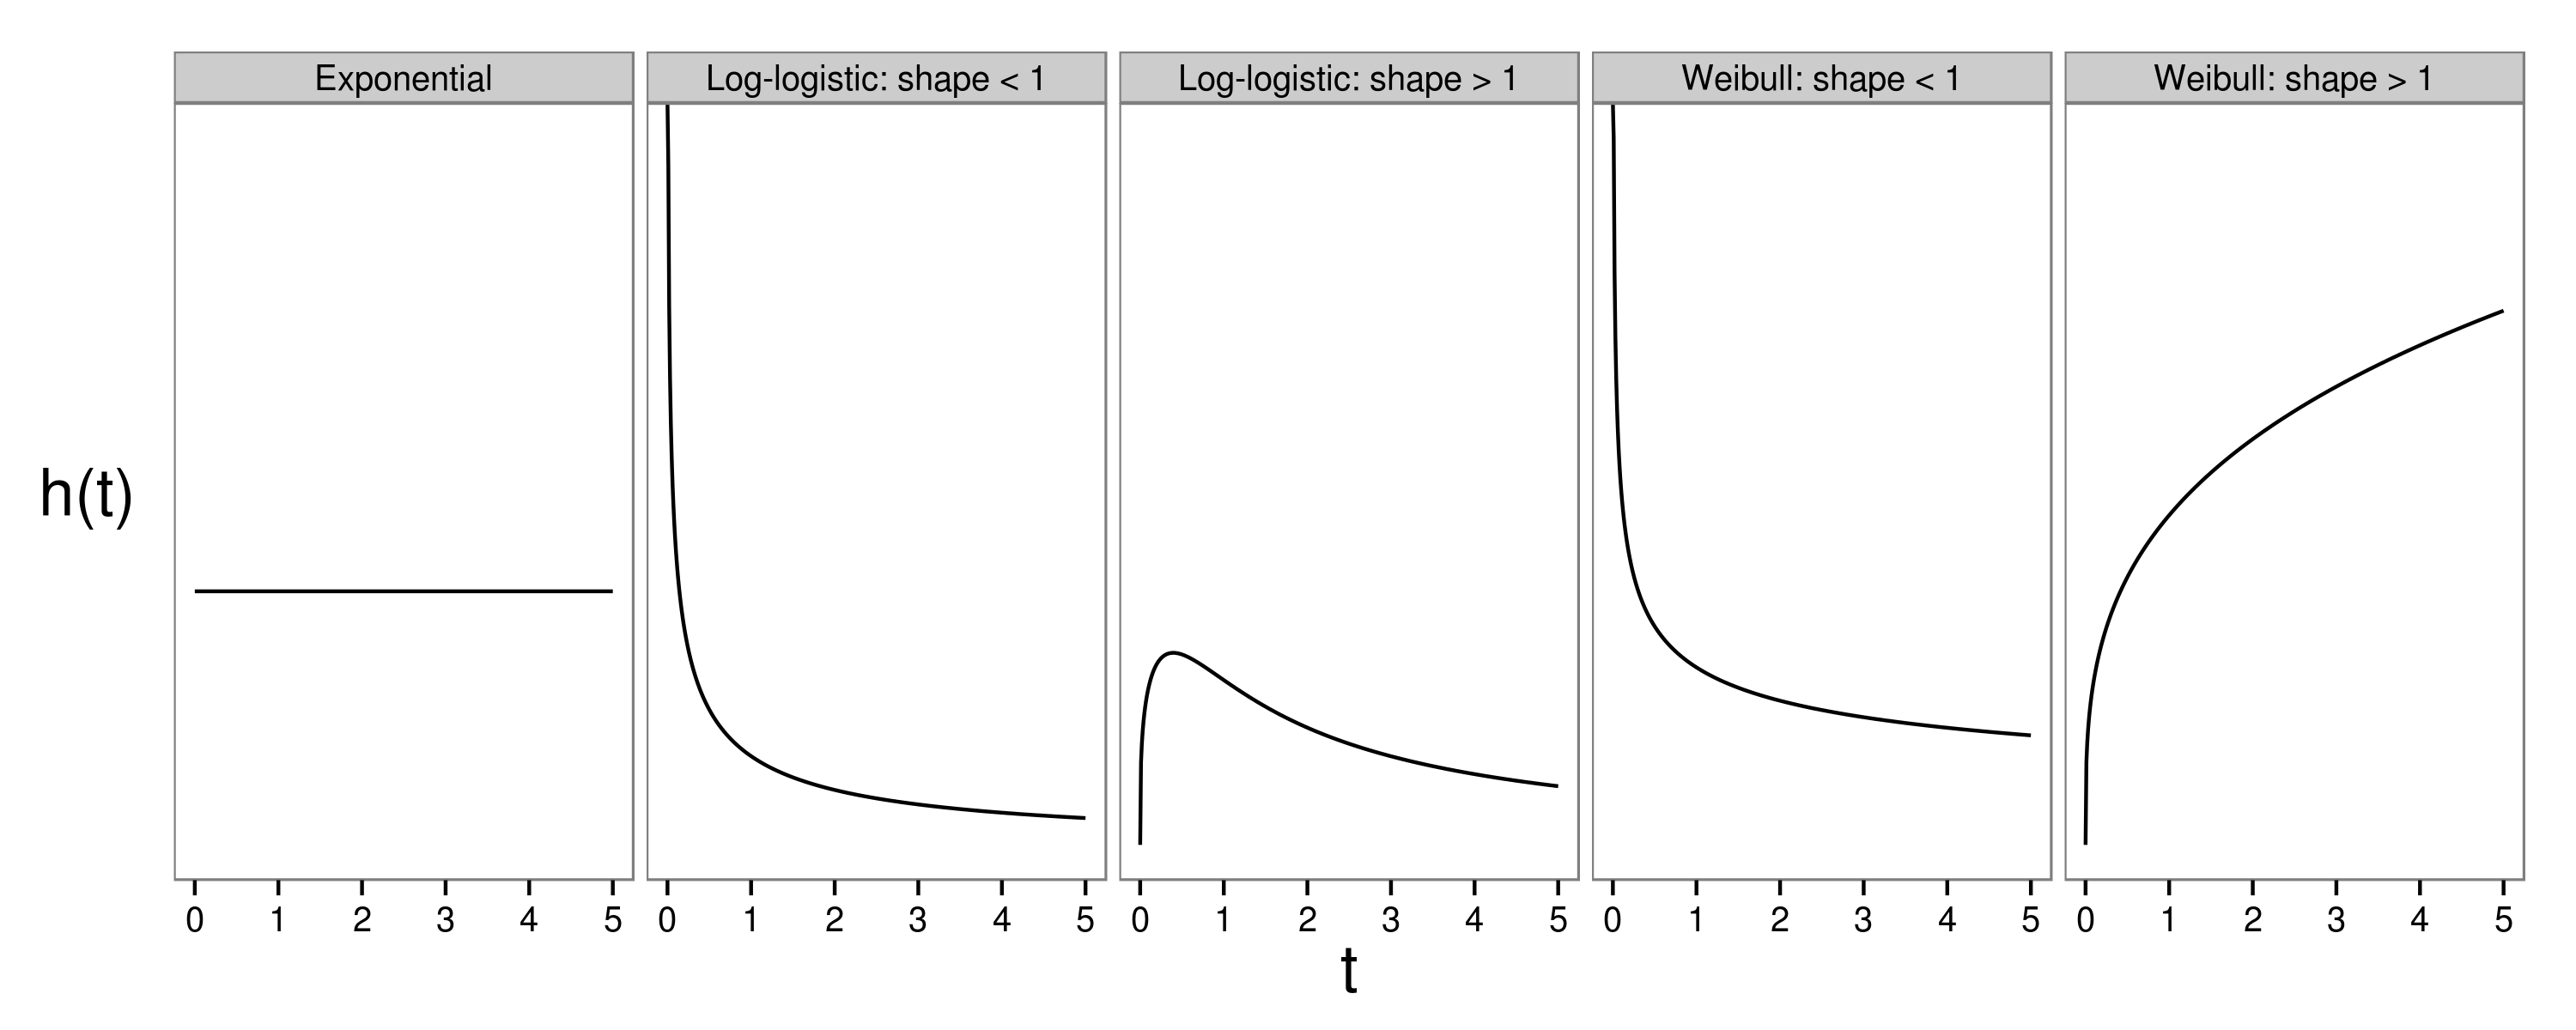
\includegraphics[width = \textwidth, keepaspectratio = true]{figure/hazard}
  \end{center}

\end{frame}

\begin{frame}
  \frametitle{Formalization of Van Valen}

  \begin{block}{Law of Constant Extinction}
    \begin{center}
      \begin{tabular}{@{}l@{}}\(T \sim Exp(\lambda)\)\end{tabular}
      \hspace{1.5cm}
      \begin{tabular}{@{}l@{}}\(T\): survival time\\\(\lambda\): expected number of \\extinctions per unit time\end{tabular}
    \end{center}
  \end{block}
\end{frame}

\begin{frame}
  \frametitle{Affixing strategy}
  % just show the strategies?

  \begin{columns}
    \begin{column}{0.5\textwidth}
      \begin{center}
        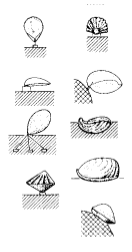
\includegraphics[height = 0.7\textheight, width = \textwidth, keepaspectratio = true]{figure/methods}

        \tiny{\attrib{modified from Johansen 1989 \textit{Paleo\(^3\)}}}
      \end{center}
    \end{column}
    \begin{column}{0.5\textwidth}
      \begin{itemize}
        \item Alexander 1977 \textit{Paleo\(^3\)}
          \begin{itemize}
            \item endemic: \\reclining \(>\) others
            \item cosmopolitan: \\ped./cement \(>\) others
          \end{itemize}
        \item Clapham and Bottjer \\2007 \textit{Paleo\(^3\)}
          \begin{itemize}
            \item pendunculate: on-shore
            \item reclining: off-shore
          \end{itemize}
      \end{itemize}
    \end{column}
  \end{columns}
\end{frame}

\begin{frame}
  \frametitle{Substrate affinity}

  \begin{columns}
    \begin{column}{0.5\textwidth}
      \begin{center}
        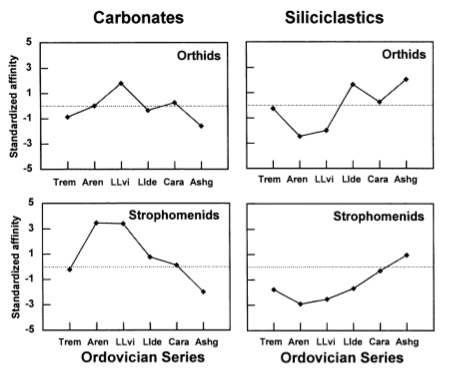
\includegraphics[width = \textwidth, keepaspectratio = true]{figure/miller}

        \tiny{\attrib{Miller and Connoly 2001 \textit{Paleobio.}}}

      \end{center}
    \end{column}
    \begin{column}{0.5\textwidth}
      \begin{center}
        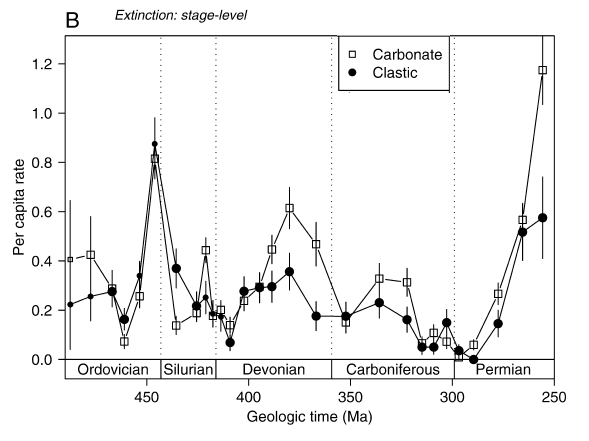
\includegraphics[width = \textwidth, keepaspectratio = true]{figure/foote}

        \tiny{\attrib{Foote 2006 \textit{Paleobio.}}}
      \end{center}
    \end{column}
  \end{columns}
\end{frame}

\begin{frame}
  \frametitle{Habitat preference}
  \begin{center}
    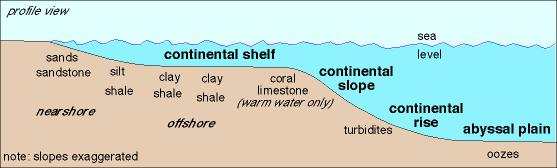
\includegraphics[height = 0.8\textheight, width = \textwidth, keepaspectratio = true]{figure/coast_dep}

    \tiny{\attrib{\url{http://www.columbia.edu/}}}
  \end{center}
\end{frame}

\begin{frame}
  \frametitle{Assigning substrate and habitat}

  \begin{block}{Probability of assignment}
    \begin{align*}
      P(H_{1}|E) &= \frac{P(E|H_{1})P(H_{1})}{P(E|H_{1})P(H_{1}) + P(E|H_{2})P(H_{2})} \\
      P(E|H) &= \binom{n}{k} p^{k}(1 - p)^{n - k}
    \end{align*}

    \begin{itemize}
      \item \(p\): proportion of all collections (e.g) carbonate
      \item \(n\): total \# taxon occurrences
      \item \(k\): of \(n\), \# (e.g.) carbonate occurrences
    \end{itemize}
  \end{block}
  
  \tiny{\attrib{Simpson and Harnik 2009 \textit{Paleobiology}}}
\end{frame}

\begin{frame}
  \frametitle{Analysis}
  \begin{columns}
    \begin{column}{0.6\textwidth}
      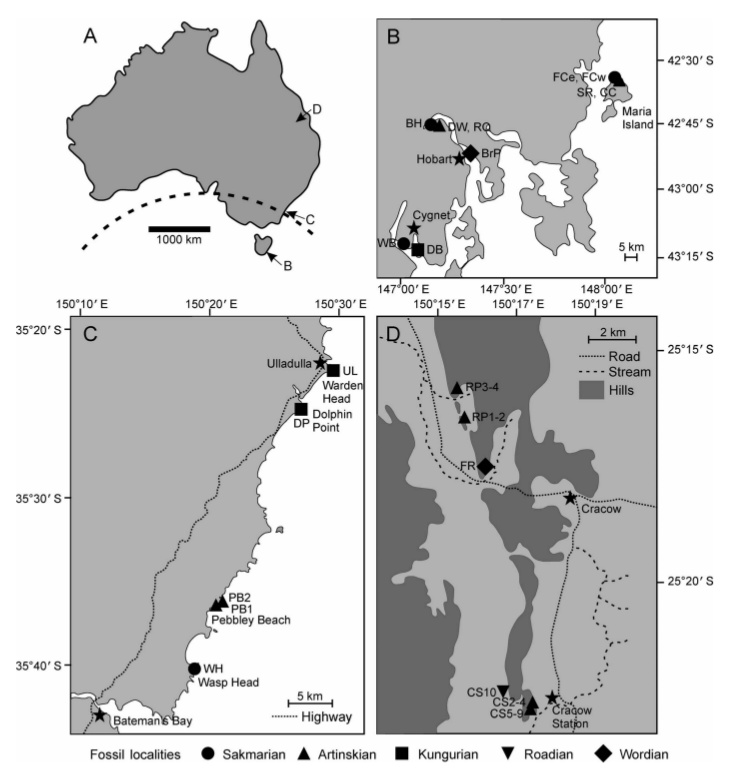
\includegraphics[height = 0.8\textheight, width = \textwidth, keepaspectratio = true]{figure/australia}

      \tiny{\attrib{Clapham and James 2008 \textit{Palaios}}}
    \end{column}
    \begin{column}{0.4\textwidth}
      \begin{itemize}
        \item age \(\sim\) Exponential or Weibull 
        \item \(\lambda \propto\) interactions, \\\(k\) constant
        \item range in/out taxa right censored
        \item habitat, substrate unedited from PBDB \\(this analysis)
      \end{itemize}
    \end{column}
  \end{columns}
\end{frame}

\begin{frame}
  \frametitle{K-M curve habitat}
  \begin{center}
    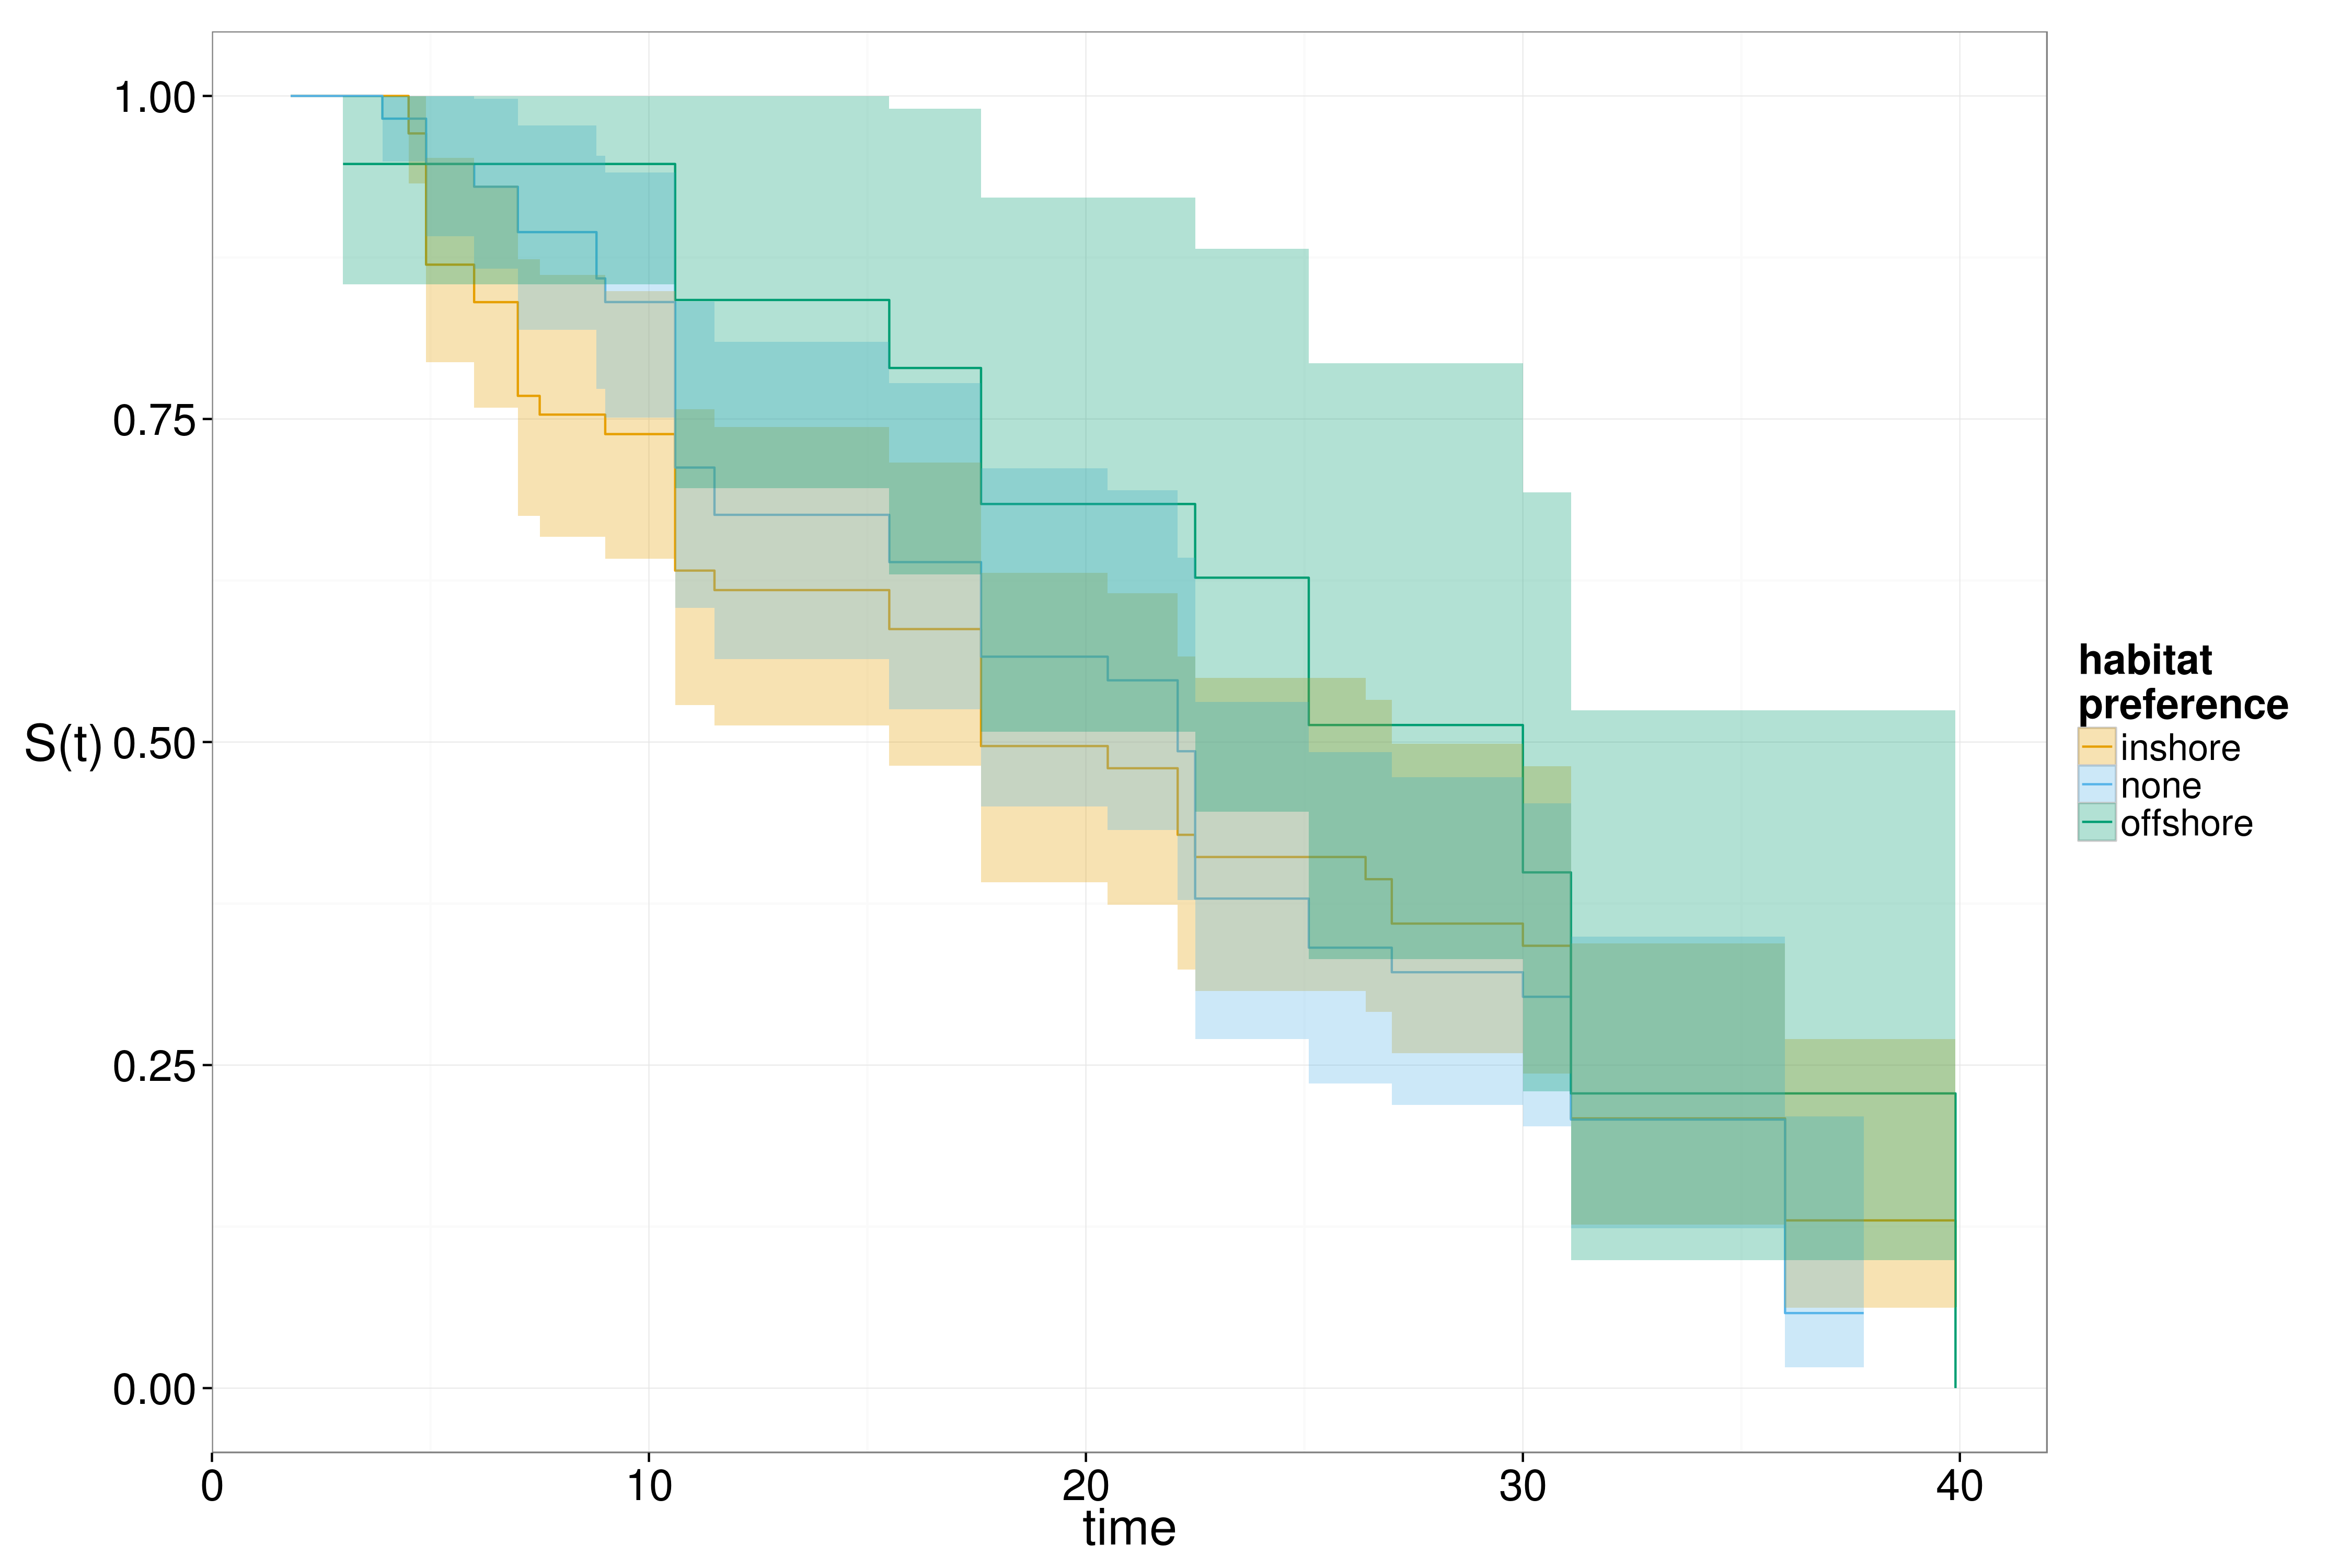
\includegraphics[height = 0.8\textheight, width = \textwidth, keepaspectratio = true]{figure/km_hab}
  \end{center}
\end{frame}

\begin{frame}
  \frametitle{K-M curve substrate}
  \begin{center}
    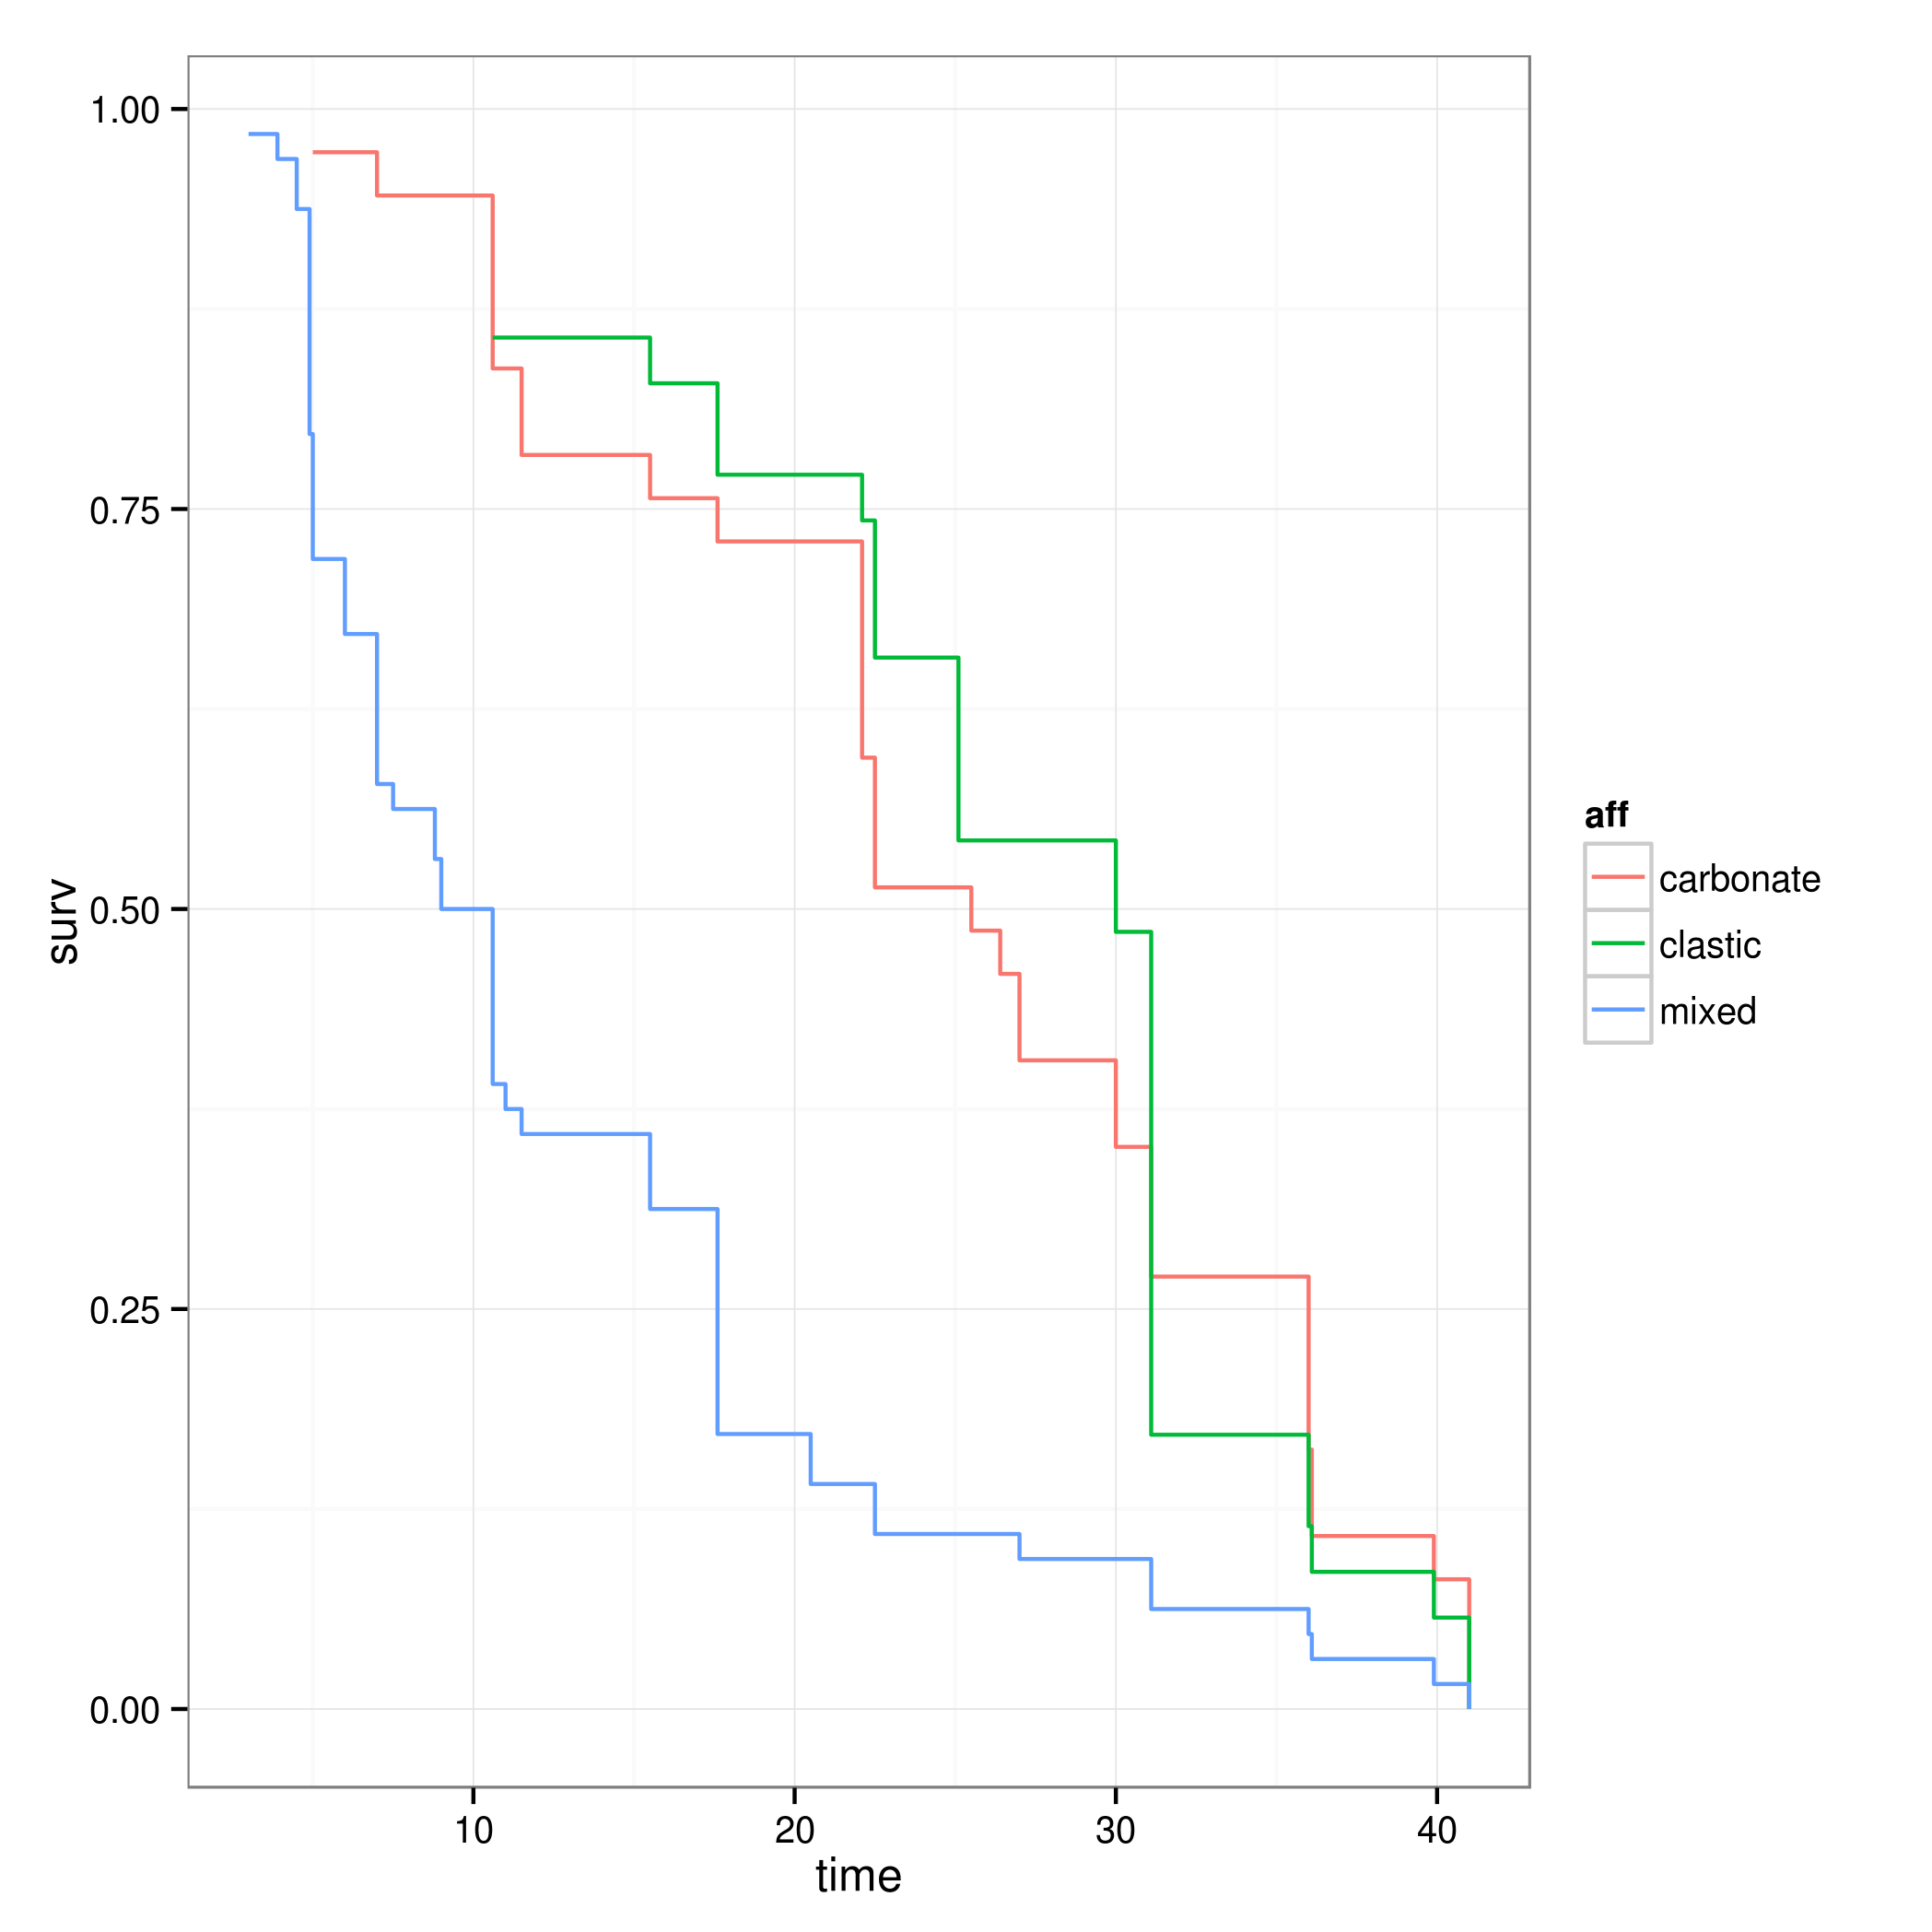
\includegraphics[height = 0.8\textheight, width = \textwidth, keepaspectratio = true]{figure/km_aff}
  \end{center}
\end{frame}

\begin{frame}
  \frametitle{Preliminary results: model comparison}

  % latex table generated in R 3.0.2 by xtable 1.7-1 package
% Thu Jan  9 14:42:10 2014
\begin{table}[ht]
\centering
\begin{tabular}{llrrrr}
 formula & distribution & shape & df & logLik & AICc \\ 
  \hline
\~{} aff & weibull & 1.91 & 4 & -497.5745 & 1003.4543 \\ 
  \~{} aff + hab & weibull & 1.92 & 6 & -496.8553 & 1006.3618 \\ 
  \~{} aff * hab & weibull & 1.94 & 10 & -495.7702 & 1013.3003 \\ 
  \~{} 1 & weibull & 1.76 & 2 & -515.1666 & 1034.4234 \\ 
  \~{} hab & weibull & 1.76 & 4 & -513.9591 & 1036.2236 \\ 
  \~{} aff & exponential &  & 3 & -532.8690 & 1071.9199 \\ 
  \~{} aff + hab & exponential &  & 5 & -532.5798 & 1075.6211 \\ 
  \~{} 1 & exponential &  & 1 & -540.9218 & 1083.8734 \\ 
  \~{} aff * hab & exponential &  & 9 & -532.3099 & 1084.0485 \\ 
  \~{} hab & exponential &  & 3 & -540.2811 & 1086.7439 \\ 
  \end{tabular}
\label{tab:brach}
\end{table}

\end{frame}

\begin{frame}
  \frametitle{Estimated survival curve habitat}
  \begin{center}
    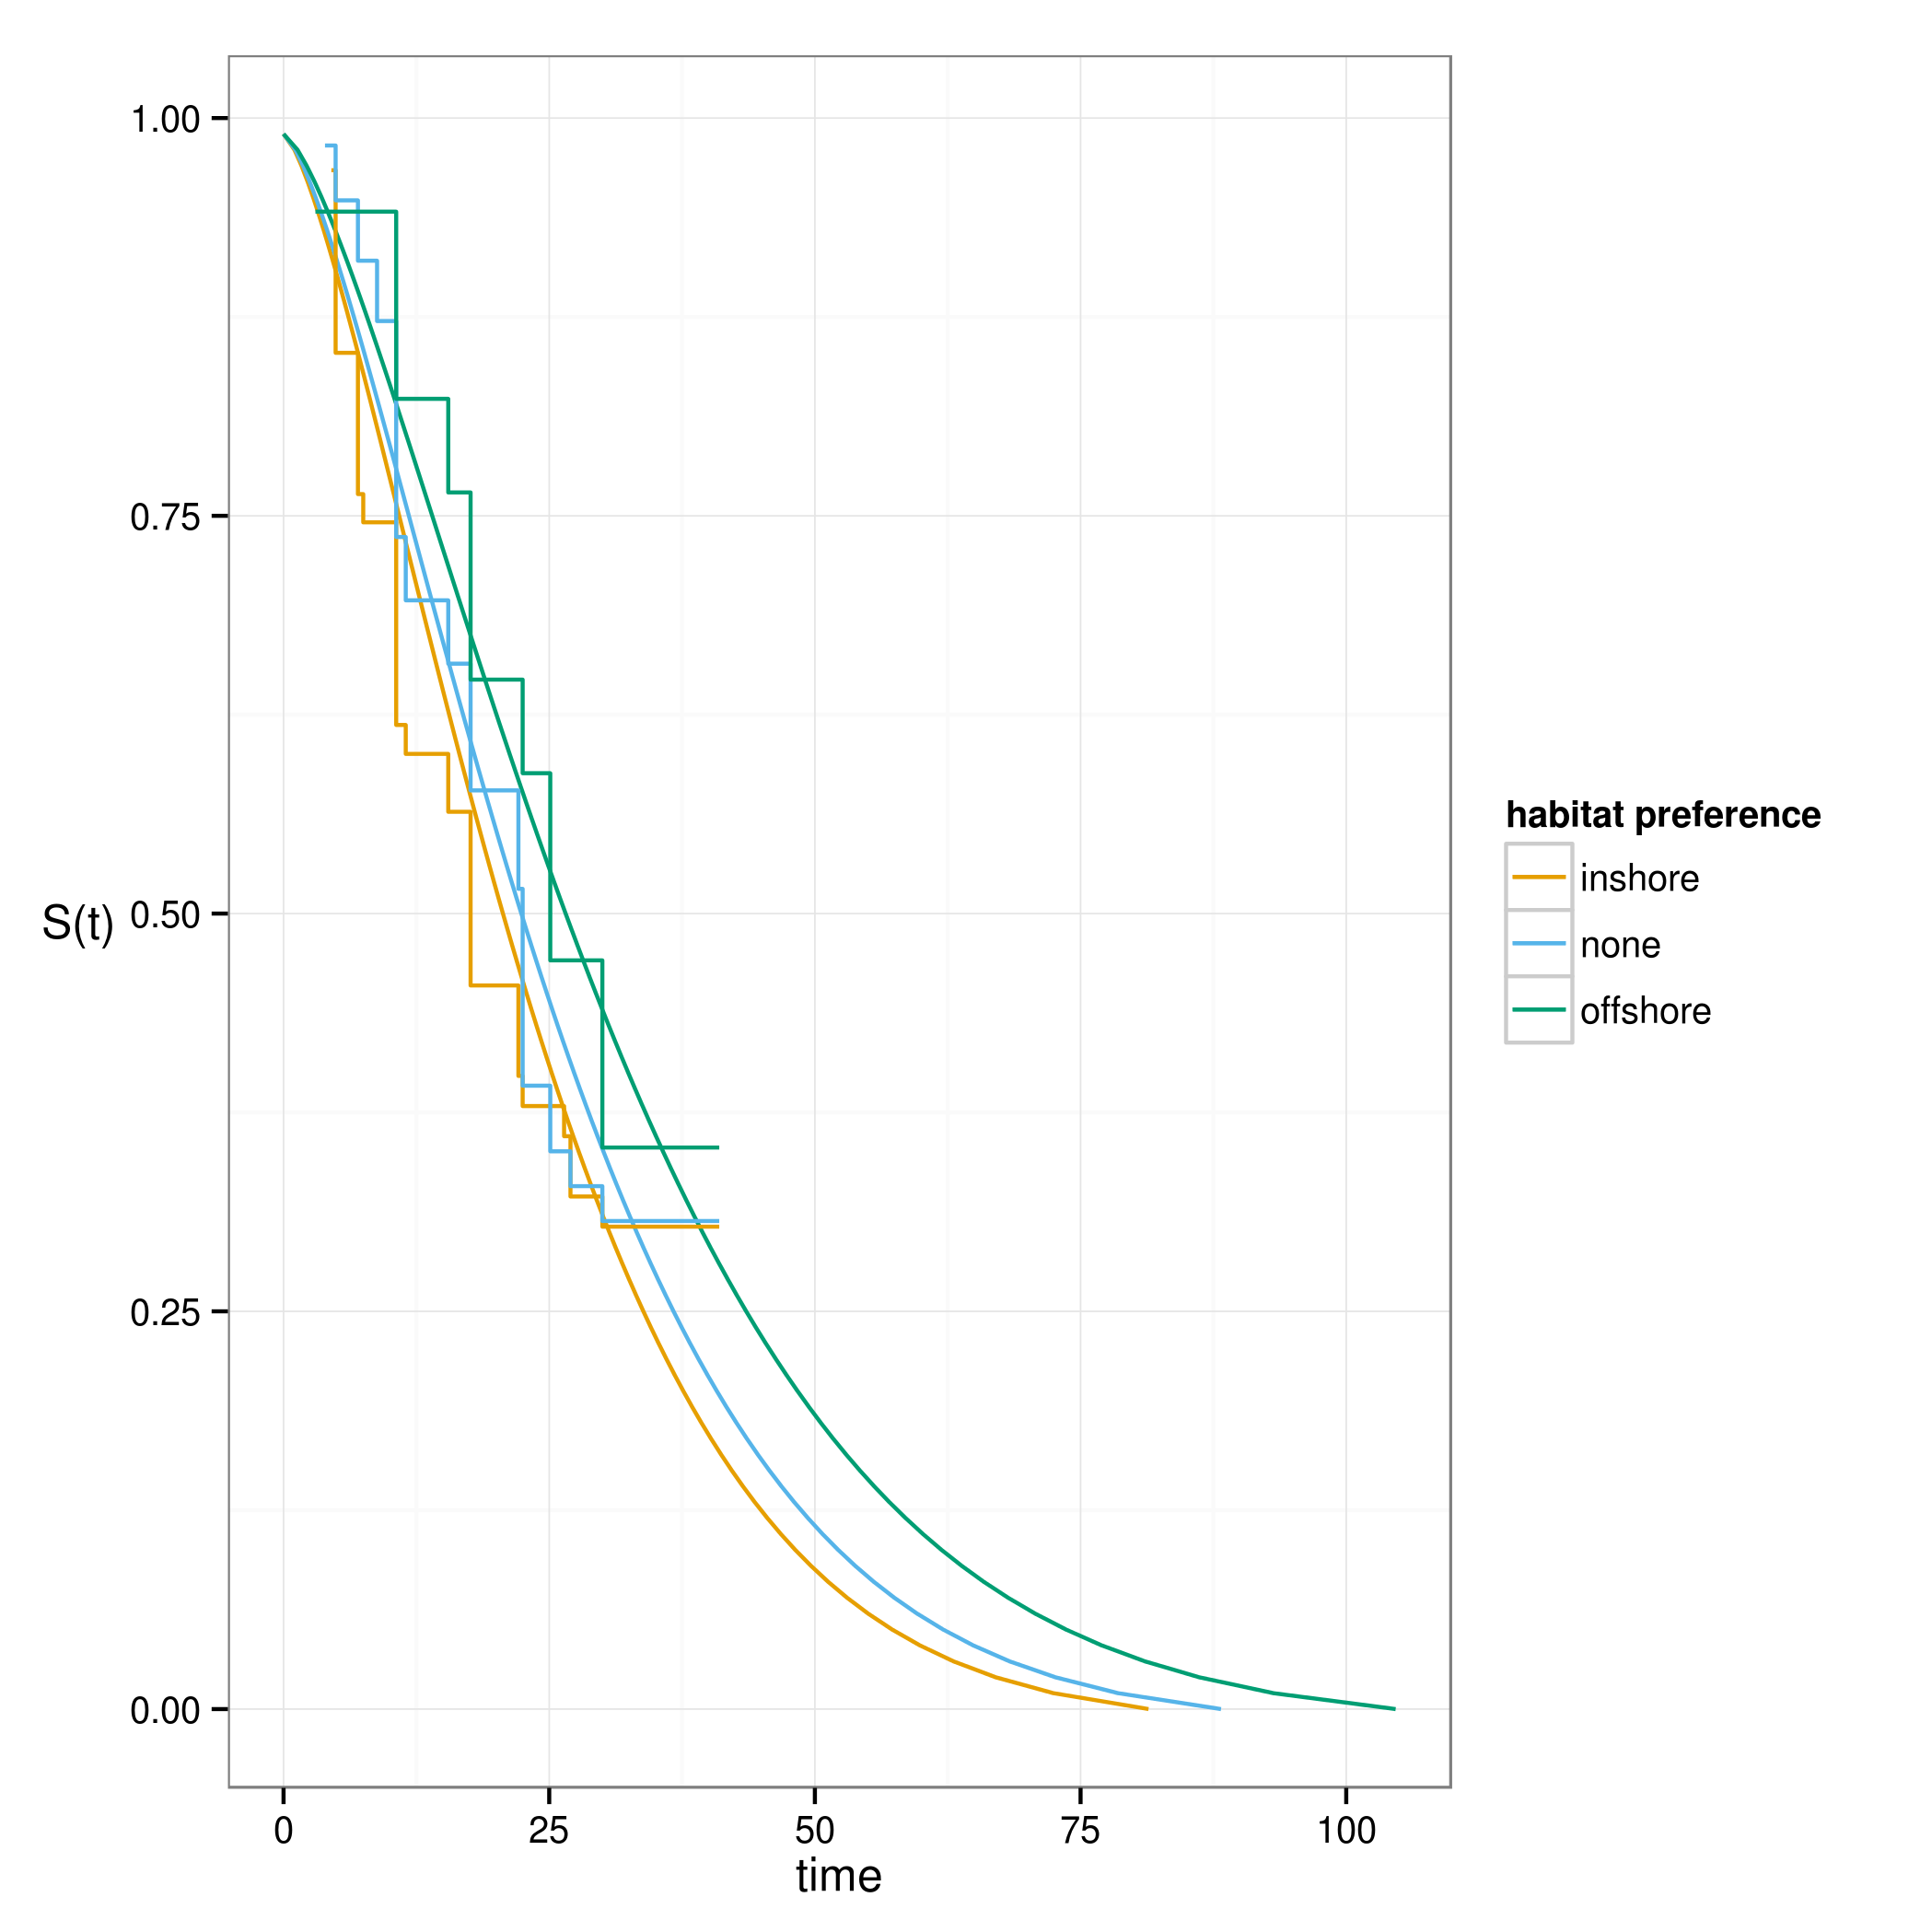
\includegraphics[height = 0.8\textheight, width = \textwidth, keepaspectratio = true]{figure/hab}
  \end{center}
\end{frame}

\begin{frame}
  \frametitle{Estimated survival curve substrate}
  \begin{center}
    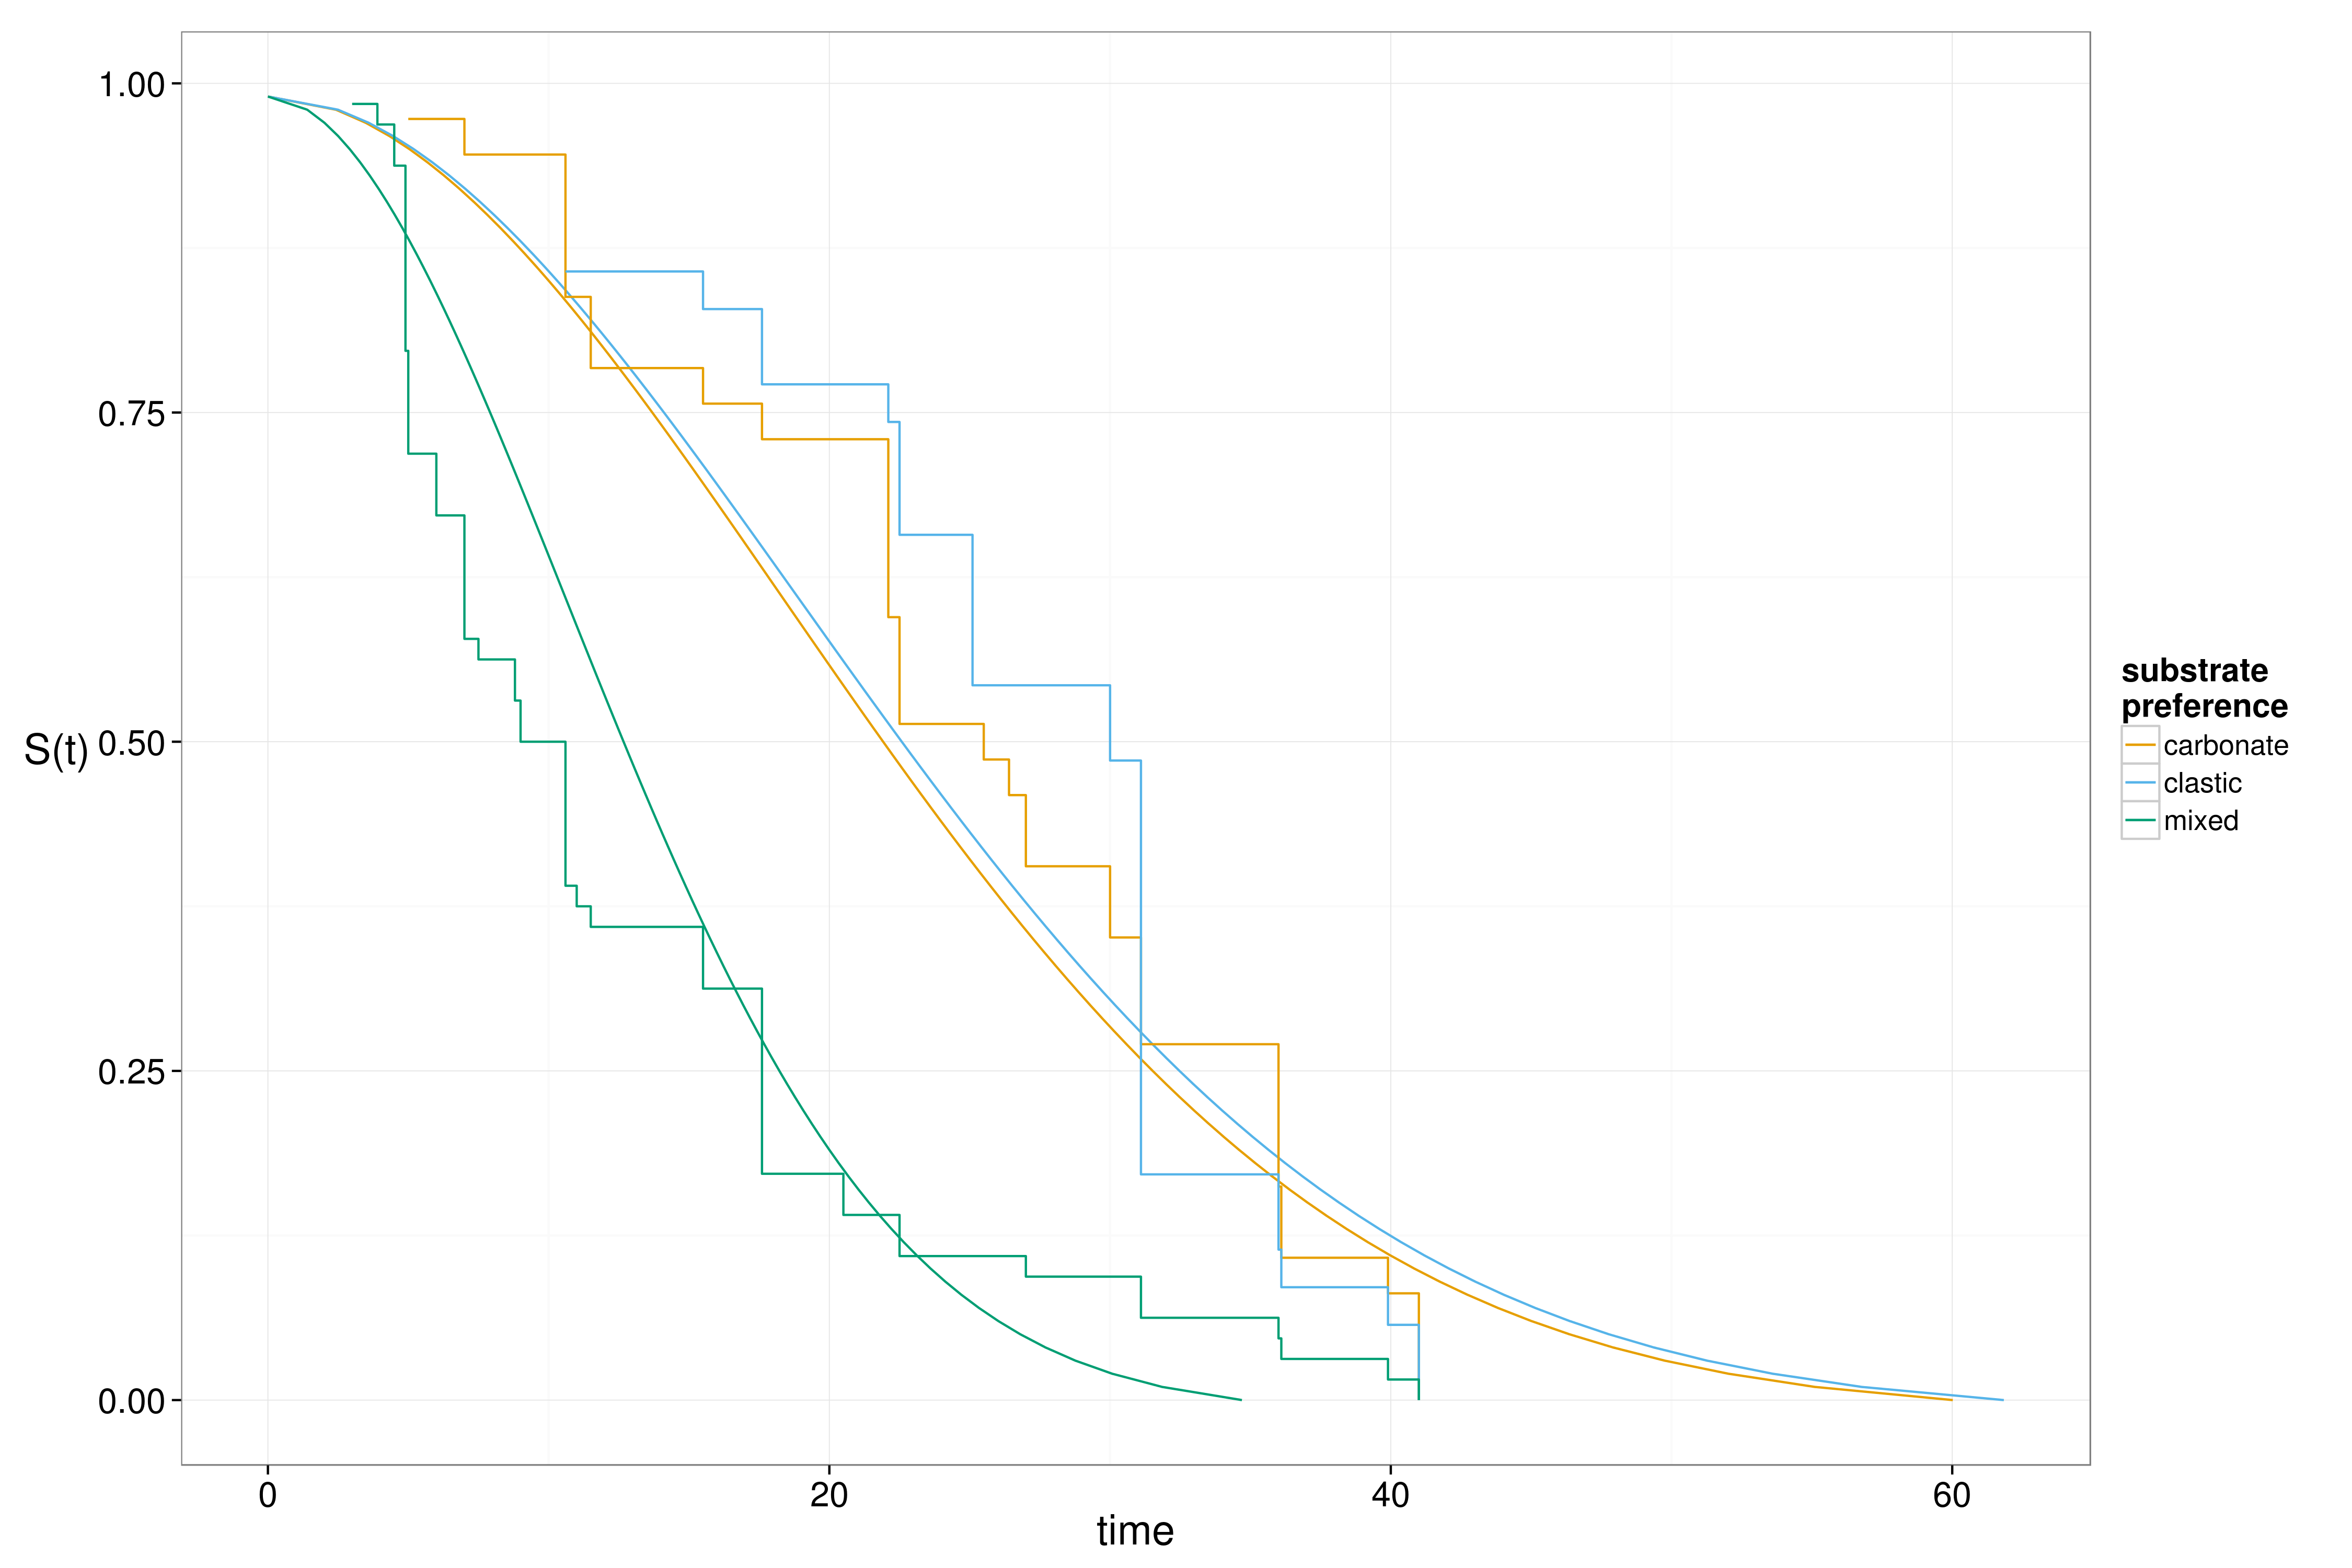
\includegraphics[height = 0.8\textheight, width = \textwidth, keepaspectratio = true]{figure/aff}
  \end{center}
\end{frame}


\section{Communities}

\begin{frame}
  \frametitle{Community connectedness}
  \begin{definition}
    The relationship between \(\alpha\), \(\beta\) diversity and provinciality.
  \end{definition}
\end{frame}

\begin{frame}
  \frametitle{Mammals}
  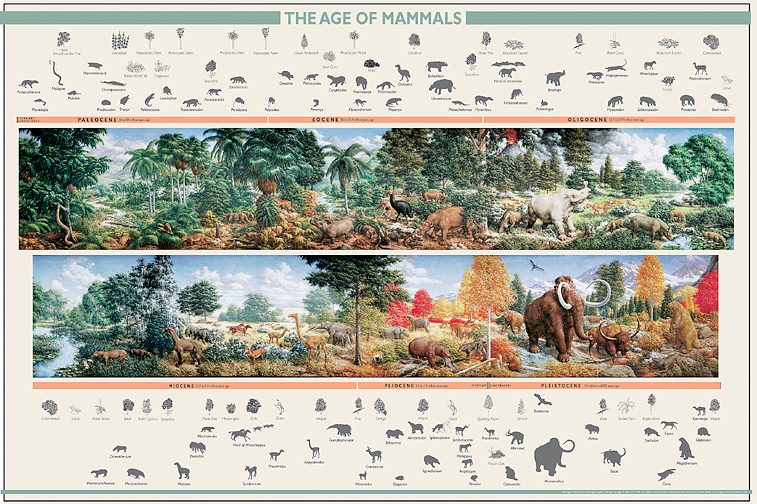
\includegraphics[height = 0.9\textheight, width = \textwidth, keepaspectratio = true]{figure/aom}

  \tiny{\attrib{Yale Peabody Museum}}
\end{frame}

\begin{frame}
  \frametitle{Community connectedness in Cenozoic mammals}

  \begin{block}{Questions}
    \begin{itemize}
      \item How does average biome \(\alpha\) and \(\beta\) diversity contribution change over time?
        \begin{itemize}
          \item Do taxa with different traits exhibit different patterns?
          \item How does this pattern vary with biome phylogenetic similarity? 
        \end{itemize}
      \item When would we expect global, regional, and/or local processes to shape taxonomic patterns?
    \end{itemize}
  \end{block}
\end{frame}

\begin{frame}
  \frametitle{Uniformity and distinctiveness}
  
  high \(\alpha\), high distinctiveness, difference in selective pressures
  
  \vspace{1cm}

  high \(\beta\), high uniformity, similarity in selective pressures

\end{frame}

\begin{frame}
  \frametitle{Environments}

  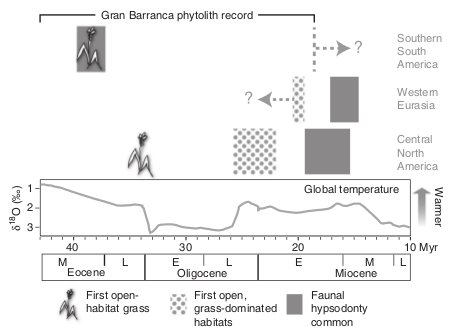
\includegraphics[height=0.8\textheight,width=\textwidth,keepaspectratio=true]{figure/stromberg}

  \tiny{\attrib{Str\"{o}mberg \textit{et al.} 2013 \textit{Nature Com.}}}
\end{frame}


\begin{frame}
  \frametitle{Occurrences}
  \begin{center}
    \textbf{A}: {2, 3, 4, 6, 7, 8}

    \vspace{0.5cm}

    \textbf{B}: {1, 3, 7, 8, 9}

    \vspace{0.5cm}

    \textbf{C}: {3, 5, 6, 7, 8}
  \end{center}

\end{frame}

\begin{frame}
  \frametitle{Biogeographic network}

  \begin{center}
    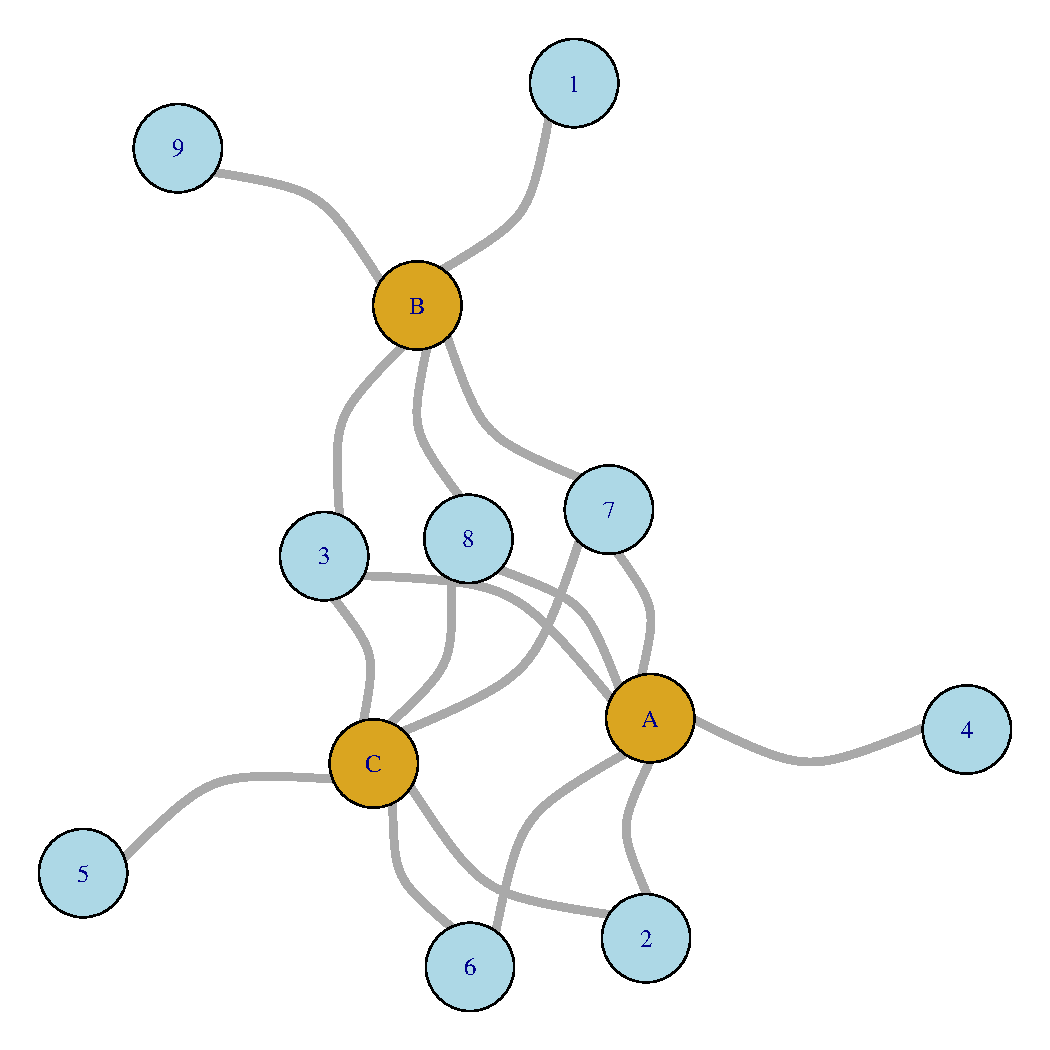
\includegraphics[height = 0.8\textheight, width = \textwidth, keepaspectratio = true]{figure/sim_graph}
  \end{center}

\end{frame}

\begin{frame}
  \frametitle{\(\alpha\) diversity}

  \begin{columns}
    \begin{column}{0.6\textwidth}
      \begin{center}
        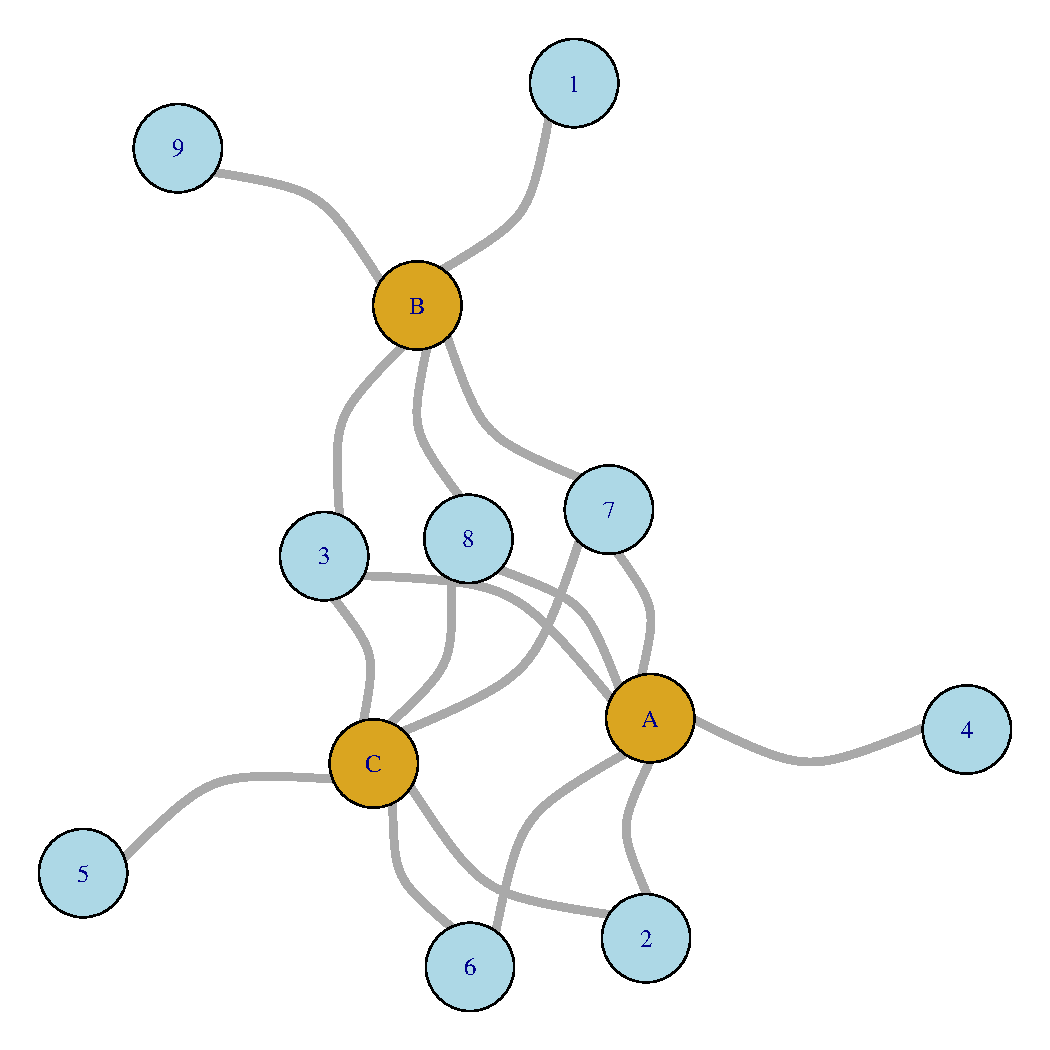
\includegraphics[height = 0.5\textheight, width = \textwidth, keepaspectratio = true]{figure/sim_graph}

        \begin{align*}
          u &= \{1, 2, 1\}\\
          n &= \{6, 5, 6\}\\
          L &= 3\\
          E &\approx 0.24
        \end{align*}
      \end{center}
    \end{column}
    \begin{column}{0.4\textwidth}
      \[
        E = \frac{\sum_{i = 1}^{L} \frac{u_{i}}{n_{i}}}{L}
      \]

      \begin{itemize}
        \item \(L\): number of localities (module)
        \item \(u\): number of taxa unique to a locality (module)
        \item \(n\): number of taxa at a locality (module)
        \item \(0 \leq E \leq 1\)
      \end{itemize}
    \end{column}
  \end{columns}
\end{frame}

\begin{frame}
  \frametitle{\(\beta\) diversity contribution}

  \begin{columns}
    \begin{column}{0.6\textwidth}
      \begin{center}
        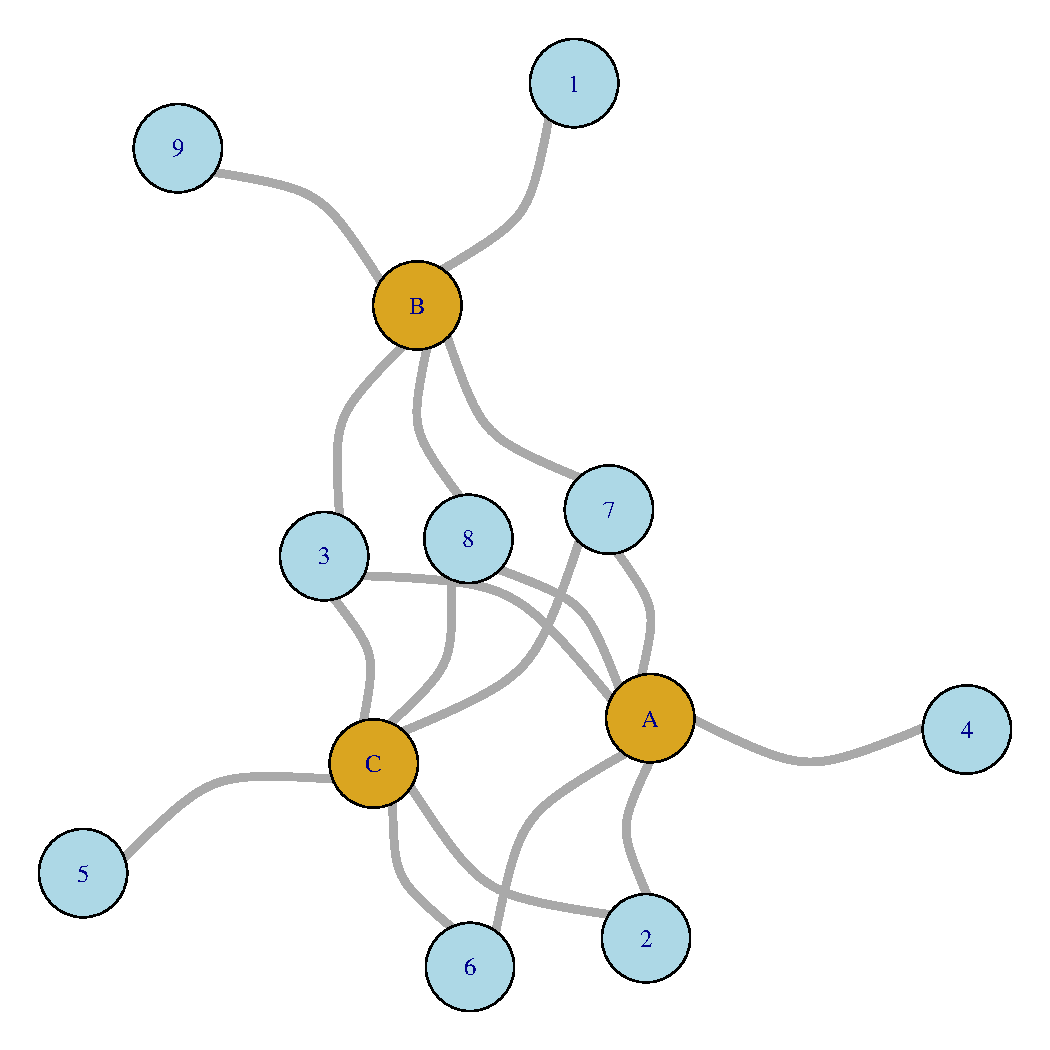
\includegraphics[height = 0.5\textheight, width = \textwidth, keepaspectratio = true]{figure/sim_graph}

        \begin{align*}
          l &= \{1, 2, 3, 1, 1, 2, 3, 3, 1\}\\
          L &= 3\\
          N &= 9\\
          Occ &\approx 0.63 
        \end{align*}
      \end{center}
    \end{column}
    \begin{column}{0.4\textwidth}
      \[
        Occ = \frac{\sum_{i = 1}^{N} \frac{l_{i}}{L}}{N}
      \]

      \begin{itemize}
        \item \(N\): total number of taxa
        \item \(l\): number of localities (module) a taxon occurs at
        \item \(L\): number of localities (module)
        \item \(0 \leq Occ \leq 1\)
      \end{itemize}
    \end{column}
  \end{columns}
\end{frame}

\begin{frame}
  \frametitle{Uniformity}

  \begin{columns}
    \begin{column}{0.6\textwidth}
      \begin{center}
        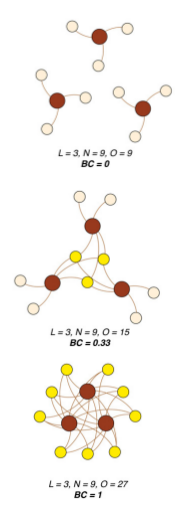
\includegraphics[height=0.8\textheight,width=\textwidth,keepaspectratio=true]{figure/bc}

        \tiny{\attrib{Sidor et al. 2013 \textit{PNAS}}}
      \end{center}
    \end{column}
    \begin{column}{0.4\textwidth}
      \[
        BC = \frac{O - N}{LN - N}
      \]

      \begin{itemize}
        \item \(O\): number of occurrences
        \item \(N\): total number of taxa
        \item \(L\): number of localities
        \item \(0 \leq BC \leq 1\)
      \end{itemize}
    \end{column}
  \end{columns}
\end{frame}

\begin{frame}
  \frametitle{Code length}
  \begin{center}
    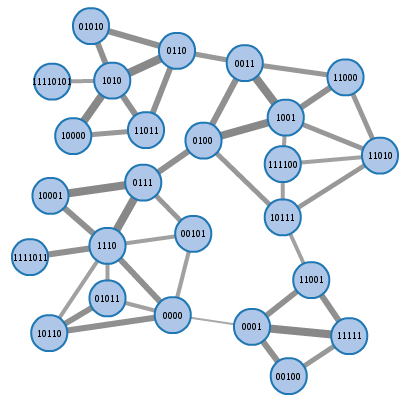
\includegraphics[height=0.8\textheight,width=\textwidth,keepaspectratio=true]{figure/network_plain}

    \tiny{\attrib{\url{mapequation.org}}}
  \end{center}
\end{frame}

\begin{frame}
  \frametitle{Code length}
  \begin{center}
    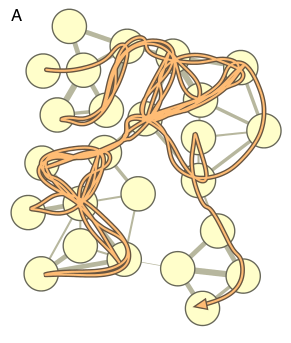
\includegraphics[height=0.8\textheight,width=\textwidth,keepaspectratio=true]{figure/map1}

    \tiny{\attrib{Rosvall and Bergstrom 2008 \textit{PNAS}}}
  \end{center}
\end{frame}

\begin{frame}
  \frametitle{Code length}
  \begin{center}
    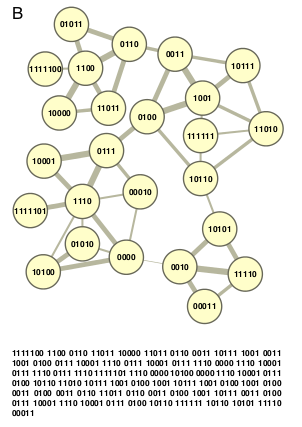
\includegraphics[height=0.8\textheight,width=\textwidth,keepaspectratio=true]{figure/map2}

    \tiny{\attrib{Rosvall and Bergstrom 2008 \textit{PNAS}}}
  \end{center}
\end{frame}

\begin{frame}
  \frametitle{Code length}
  \begin{center}
    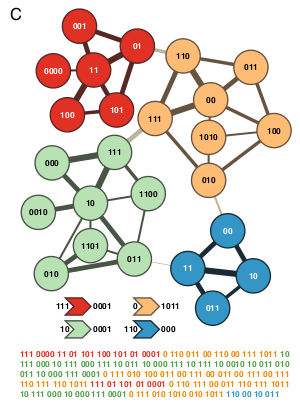
\includegraphics[height=0.8\textheight,width=\textwidth,keepaspectratio=true]{figure/map3}

    \tiny{\attrib{Rosvall and Bergstrom 2008 \textit{PNAS}}}
  \end{center}
\end{frame}

\begin{frame}
  \frametitle{Code length}
  \begin{center}
    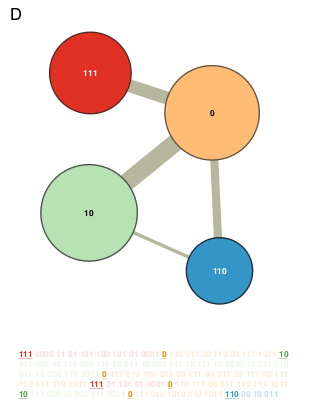
\includegraphics[height=0.8\textheight,width=\textwidth,keepaspectratio=true]{figure/map4}

    \tiny{\attrib{Rosvall and Bergstrom 2008 \textit{PNAS}}}

  \end{center}
\end{frame}

\begin{frame}
  \frametitle{Process scale}

  \begin{columns}
    \begin{column}{0.55\textwidth}
      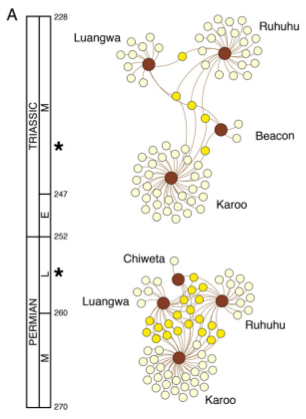
\includegraphics[height=0.7\textheight,width=\textwidth,keepaspectratio=true]{figure/permian}

      \tiny{\attrib{Sidor et al. 2013 \textit{PNAS}}}
    \end{column}
    \begin{column}{0.45\textwidth}
      \begin{itemize}
        \item global
          \begin{itemize}
            \item corr w/ global climate
            \item multiple regions corr
          \end{itemize}
        \item regional
          \begin{itemize}
            \item \(\downarrow E\), \(\uparrow Occ\), \\\(\uparrow BC\), \(\uparrow\) code
          \end{itemize}
        \item local
          \begin{itemize}
            \item \(\uparrow E\), \(\downarrow Occ\), \\\(\downarrow BC\), \(\downarrow\) code
          \end{itemize}
        \item \alert{not mutually exclusive}
      \end{itemize}
    \end{column}
  \end{columns}
\end{frame}

\begin{frame}
  \frametitle{Scenario}
  \begin{columns}
    \begin{column}{0.5\textwidth}
      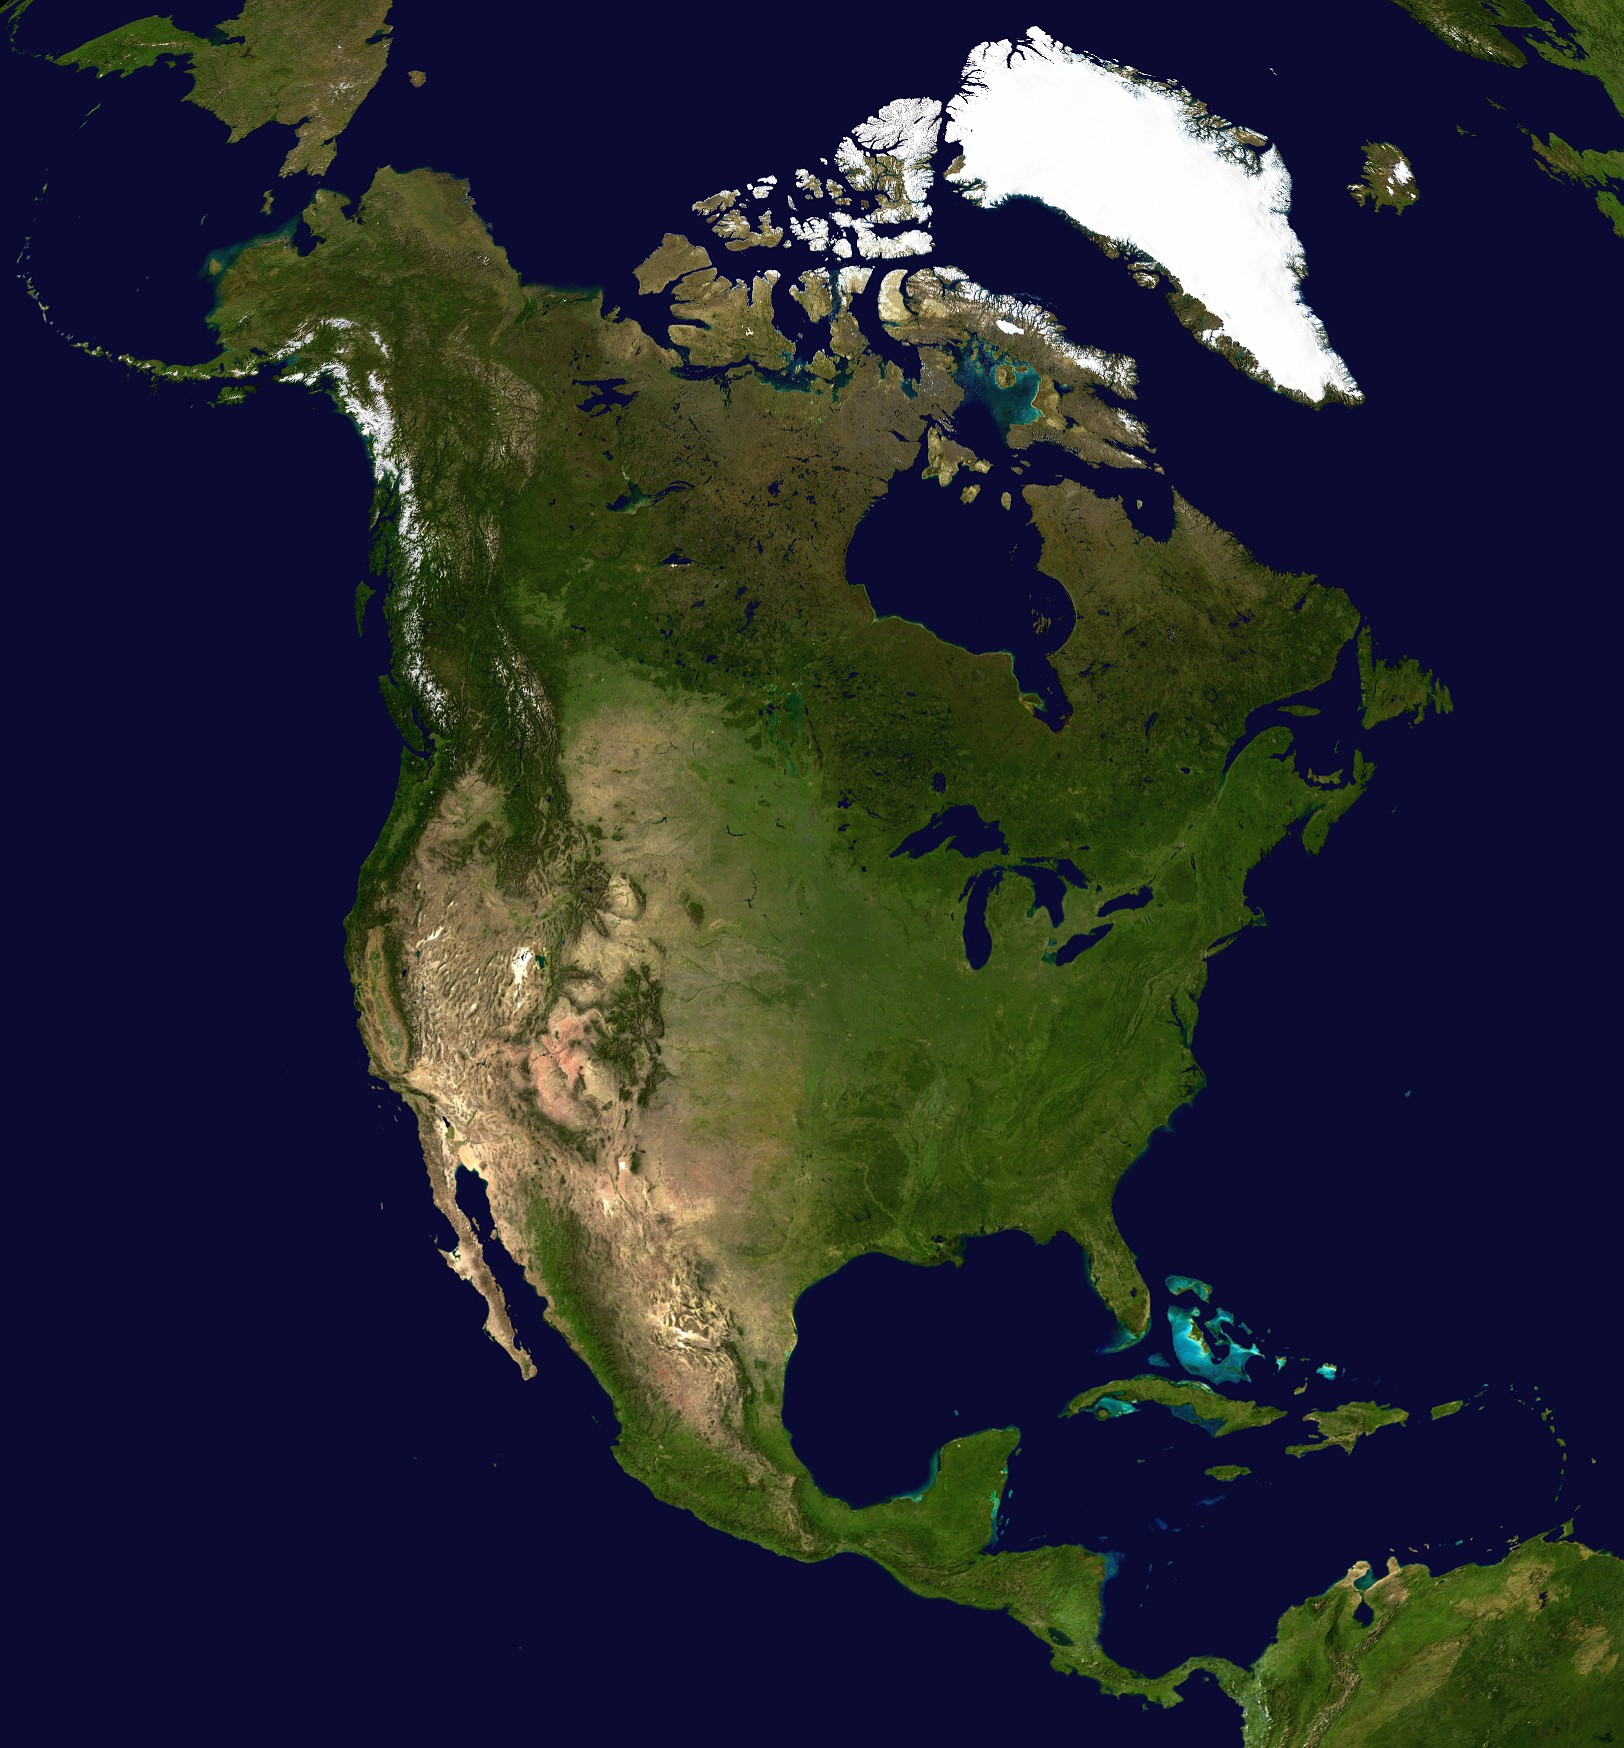
\includegraphics[height=0.5\textheight,width=\textwidth,keepaspectratio=true]{figure/na_map}
    \end{column}
    \begin{column}{0.5\textwidth}
      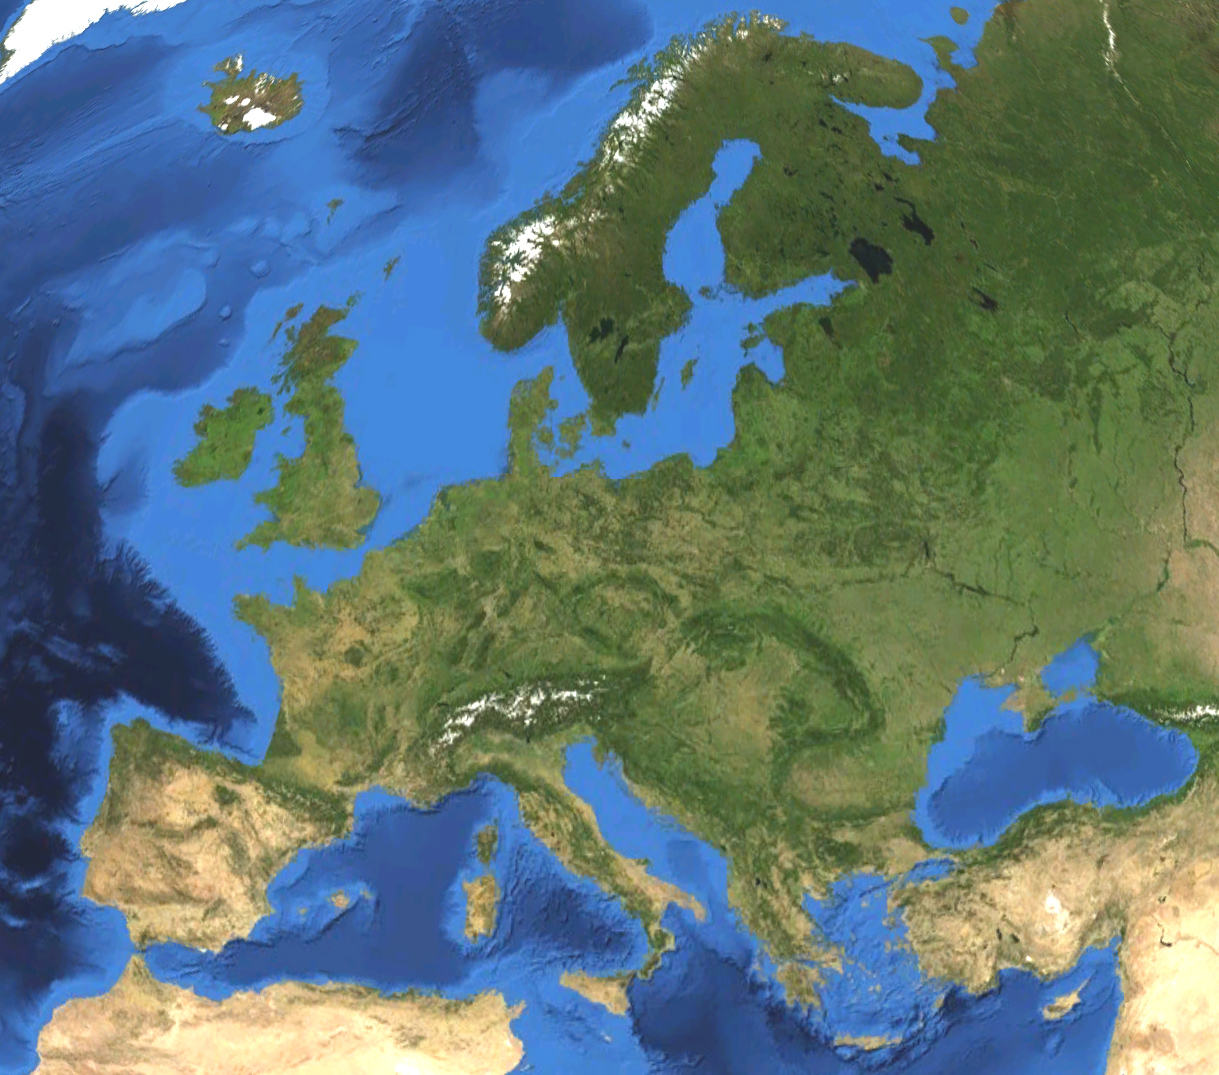
\includegraphics[height=0.7\textheight,width=\textwidth,keepaspectratio=true]{figure/euro}
    \end{column}
  \end{columns}

  \vspace{0.2cm}

  \begin{columns}
    \begin{column}{0.5\textwidth}
      Locomotor
      \begin{itemize}
        \item ground dwelling, \\arboreal, scansorial
      \end{itemize}
    \end{column}
    \begin{column}{0.5\textwidth}
      Dietary
      \begin{itemize}
        \item carnivore, insectivore, herbivore, omnivore
      \end{itemize}
    \end{column}
  \end{columns}
\end{frame}

\begin{frame}
  \frametitle{Preliminary results: NA, Eur}

  \begin{center}
    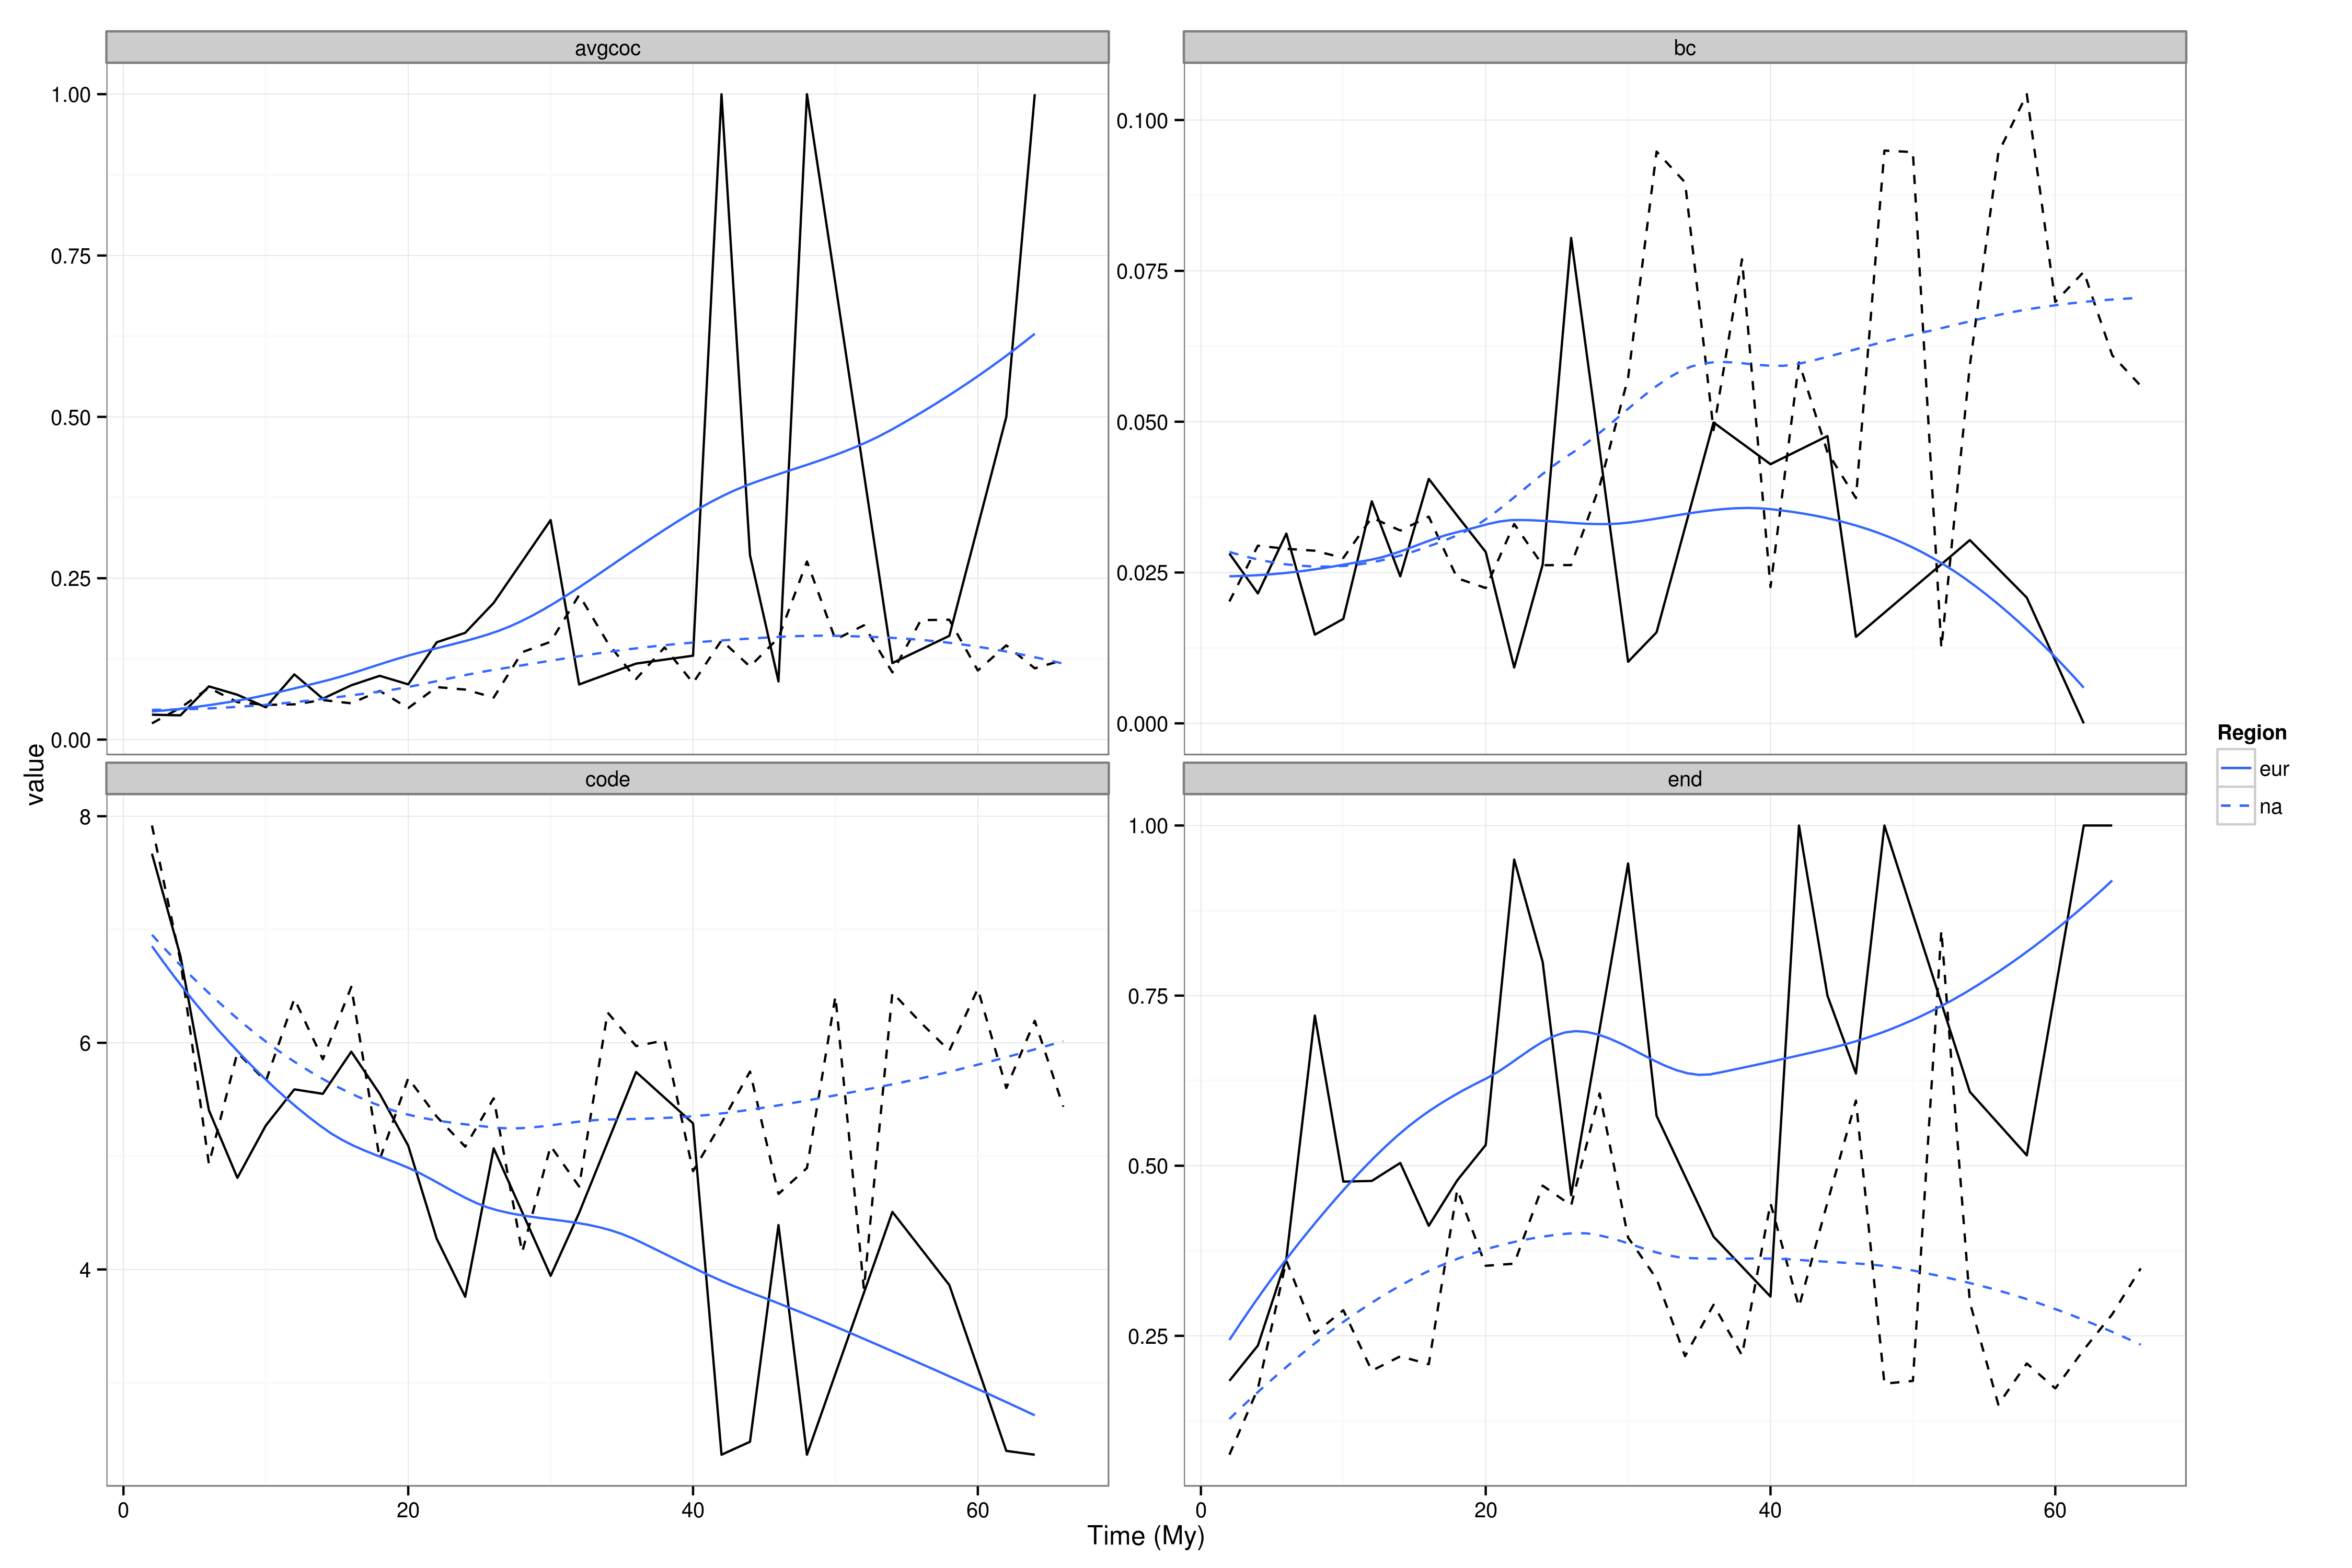
\includegraphics[height = 0.8\textheight, width = \textwidth, keepaspectratio = true]{figure/gen_bin}
  \end{center}
\end{frame}

\begin{frame}
  \frametitle{Preliminary results: locomotor category}

  \begin{center}
    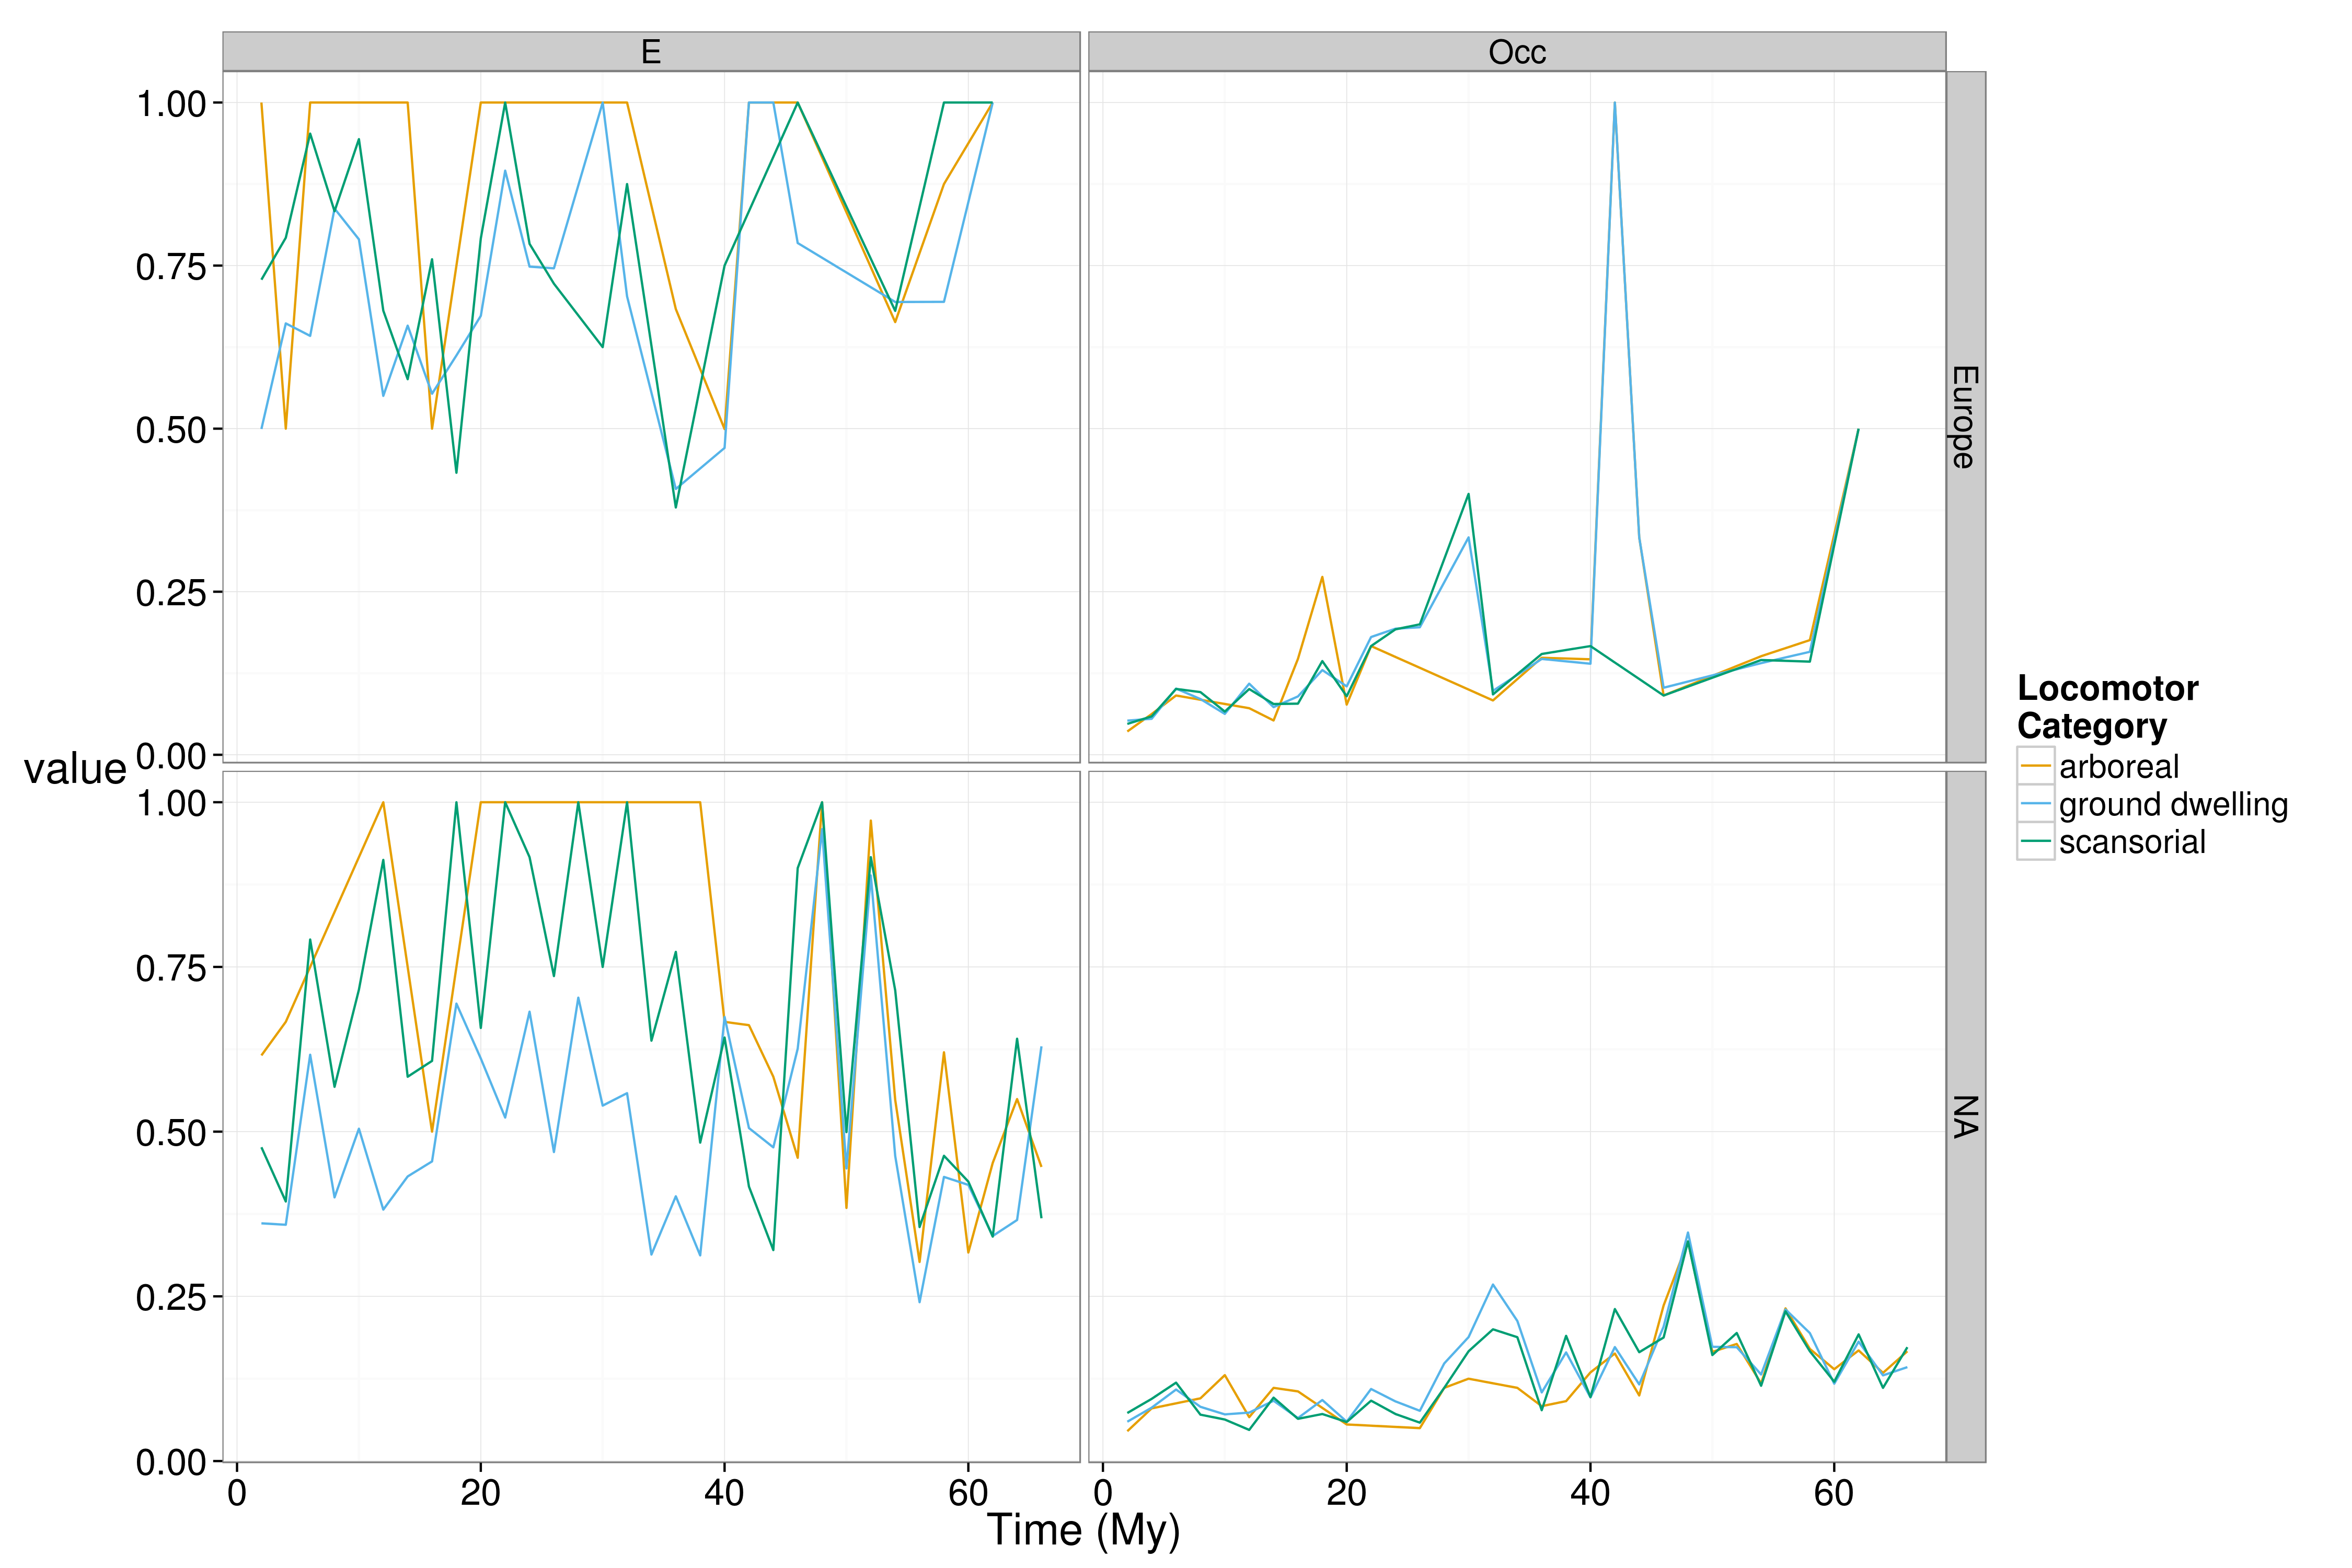
\includegraphics[height = 0.8\textheight, width = \textwidth, keepaspectratio = true]{figure/comp_loco}
  \end{center}
\end{frame}

\begin{frame}
  \frametitle{Preliminary results: dietary category}

  \begin{center}
    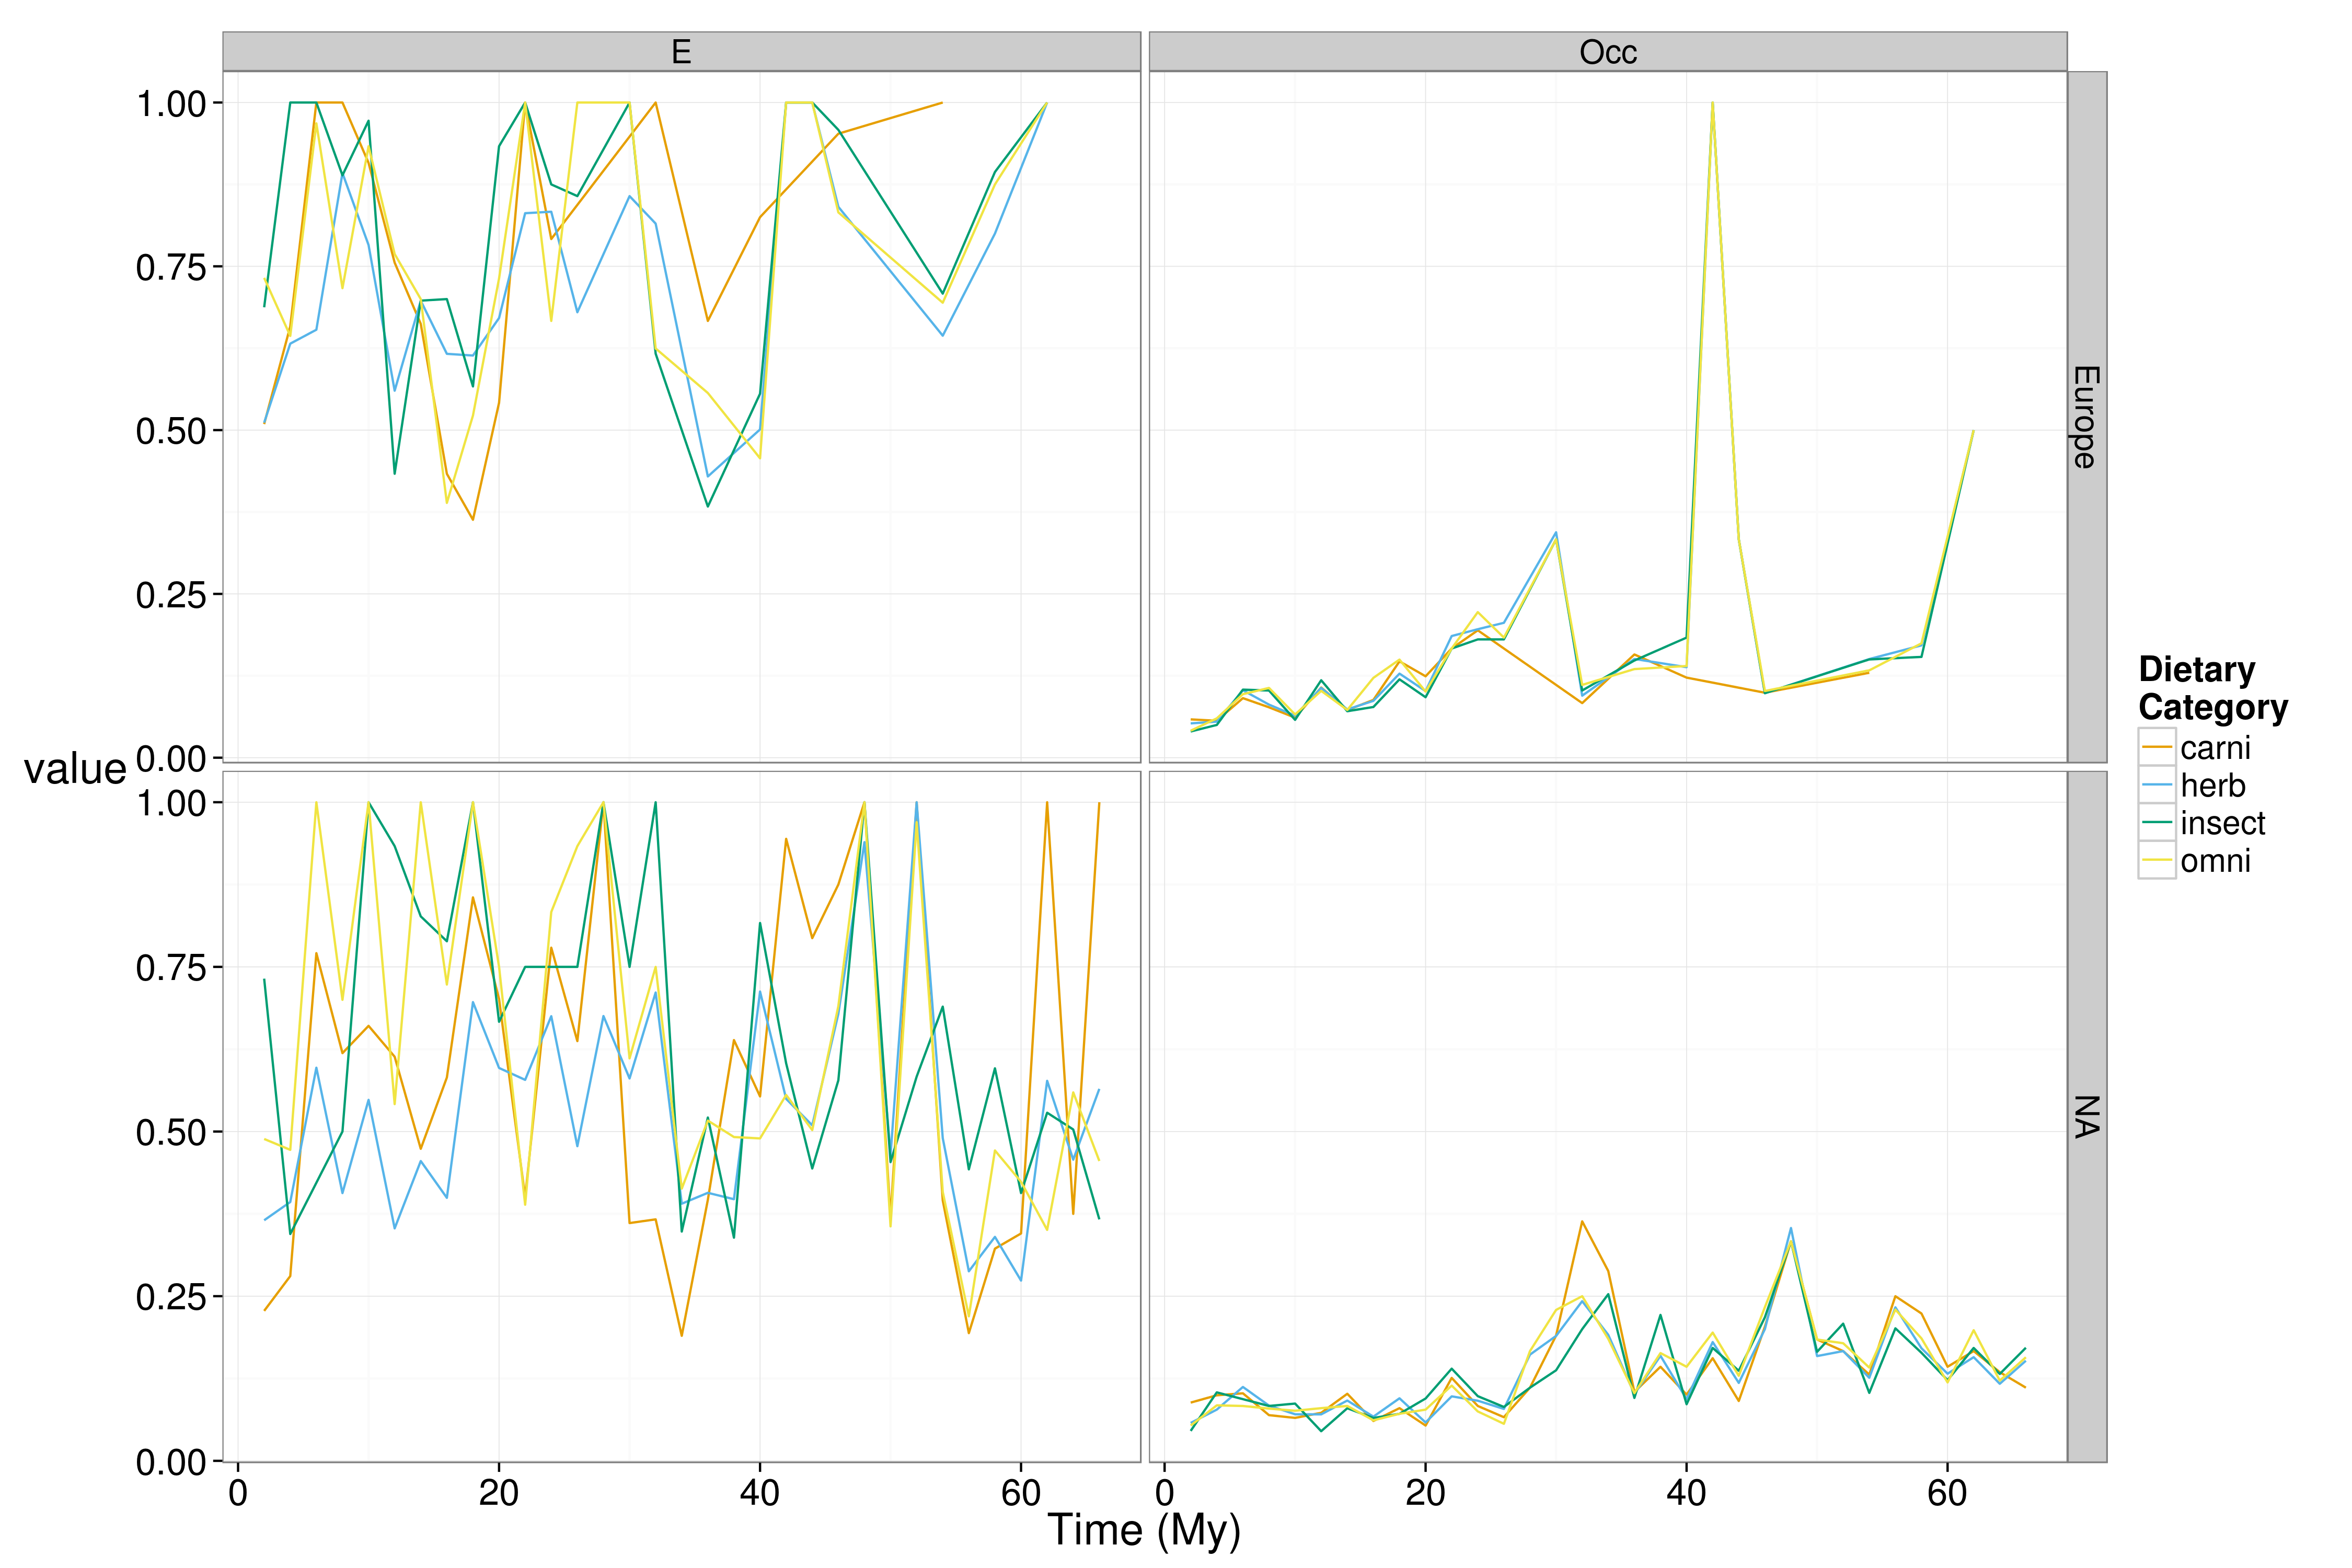
\includegraphics[height = 0.8\textheight, width = \textwidth, keepaspectratio = true]{figure/comp_diet}
  \end{center}
\end{frame}


\section{Summary}

\begin{frame}
  \frametitle{Fundamental}

  \begin{alertblock}{Question}
    Why do some taxa go extinct while others do not?
  \end{alertblock}
\end{frame}

\begin{frame}
  \frametitle{Evolutionary paleoecological rephrasing}

  \begin{block}{Question}
    How does a taxon's adaptive zone affect extinction risk?
  \end{block}
\end{frame}

\begin{frame} 
  \frametitle{Modes and patterns}

  \begin{block}{Modes of extinction \tiny{\attrib{Raup 1991 \underline{Extinction: Bad Genes or Bad Luck?}}}}
    \hspace{\stretch{0.4}} Field of Bullets 
    \hspace{\stretch{0.5}} \textbf{--} 
    \hspace{\stretch{0.5}} Wanton 
    \hspace{\stretch{0.5}} \textbf{--} 
    \hspace{\stretch{0.5}} Fair Game 
    \hspace{\stretch{1}}
  \end{block}

  \vspace{1cm}

  \begin{block}{Law of Constant Extinction \tiny{\attrib{Van Valen 1973 \textit{Evol. Theory}}}}
    Extinction risk, in a given adaptive zone, is taxon--age independent.
  \end{block}
\end{frame}

\begin{frame}
  \frametitle{Ask the following\dots}

  \begin{center}
    Is there a \alert{general pattern} of extinction?

    \vspace{0.75cm}

    \alert{What} traits matter for extinction and \alert{when}?

    \vspace{0.75cm}

    \alert{How} do traits matter for extinction?
  \end{center}
\end{frame}

\begin{frame}
  \frametitle{Acknowledgements}
  \begin{columns}
    \begin{column}{0.5\textwidth}
      \begin{itemize}
        \item \textbf{Committee}
          \begin{itemize}
            \item Kenneth D. Angielczyk (co-advisor)
            \item Michael J. Foote (co-advisor)
            \item P. David Polly
            \item Richard H. Ree
          \end{itemize}
        \item Discussion
          \begin{itemize}
            \item David Bapst, Megan Boatright, Ben Frable, Colin Kyle, Darcy Ross, Liz Sander
            \item John Alroy, Graeme Lloyd, Kathleen Ritterbush, Carl Simpson, Graham Slater
          \end{itemize}
      \end{itemize}
    \end{column}
    \begin{column}{0.5\textwidth}
      
\includegraphics[height = 0.3\textheight, keepaspectratio = true]{figure/chicago} 
      
\includegraphics[width = 0.4\textwidth, keepaspectratio = true]{figure/field}

      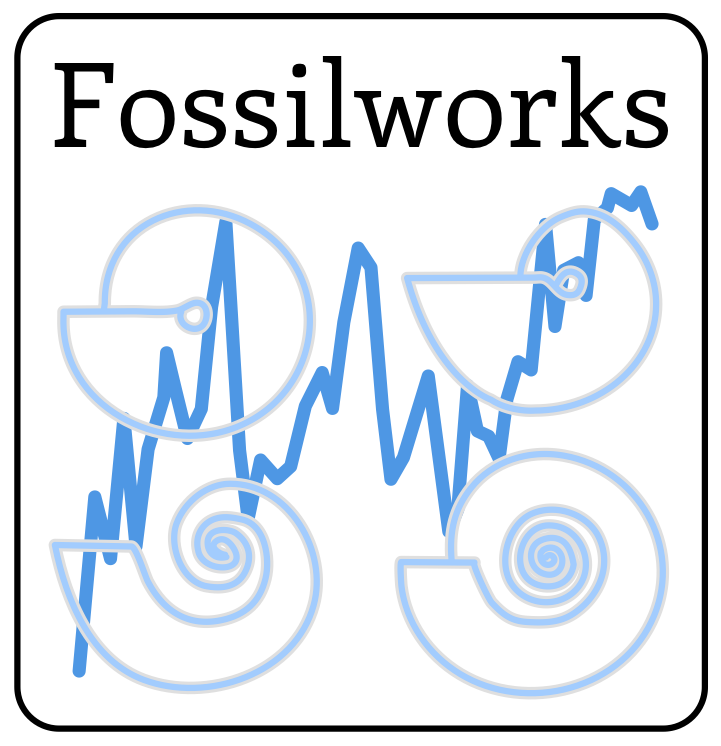
\includegraphics[height = 0.3\textheight, width = 0.5\textwidth, keepaspectratio = true]{figure/fossilworks}
      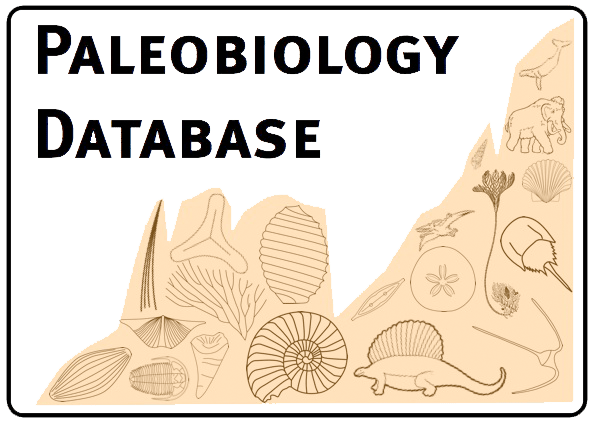
\includegraphics[width = 0.5\textwidth, keepaspectratio = true]{figure/paleodb}

      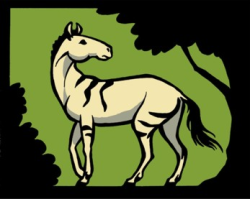
\includegraphics[height = 0.3\textheight, width = 0.5\textwidth, keepaspectratio = true]{figure/now}
    \end{column}
  \end{columns}
\end{frame}



\appendix
\section{Further concerns}

\begin{frame}
  \frametitle{Age distributions}

  \begin{columns}
    \begin{column}{0.5\textwidth}
      Exponential

      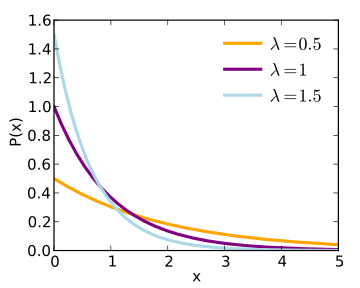
\includegraphics[height = 0.8\textheight, width = \textwidth, keepaspectratio = true]{figure/exponential}
    \end{column}
    \begin{column}{0.5\textwidth}
      Weibull

      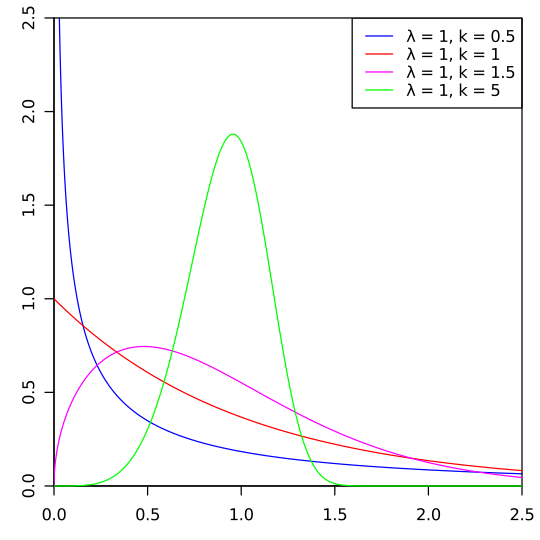
\includegraphics[height = 0.8\textheight, width = \textwidth, keepaspectratio = true]{figure/weibull}
    \end{column}
  \end{columns}
  
  \tiny{\attrib{\url{http://www.wikimedia.org/}}}
\end{frame}

\begin{frame}
  \frametitle{Algebra of age distributions}

  % weibull
  \begingroup
    \addtolength{\jot}{1em}
    \begin{align*}
      f(x; \lambda_{Weibull}, k) &= 
      \begin{cases}
        \frac{k}{\lambda} \frac{x}{\lambda}^{k - 1} \exp^{-(x / \lambda)^{k}} & x \geq 0 \\
        0 & x < 0
      \end{cases} \\
      f(x; \lambda_{\exp}) &= 
      \begin{cases}
        \lambda \exp^{- \lambda x} & x \geq 0 \\
        0 & x < 0
      \end{cases} \\
      \lambda_{Weibull} &= \frac{1}{\lambda_{\exp}} \\
      f(x; \lambda_{Weibull}, k = 1) &= f(x; \lambda_{\exp}) 
    \end{align*}
  \endgroup

\end{frame}

\begin{frame}
  \frametitle{Differential preservation and survival}

  \begin{columns}
    \begin{column}{0.5\textwidth}
      \begin{center}
        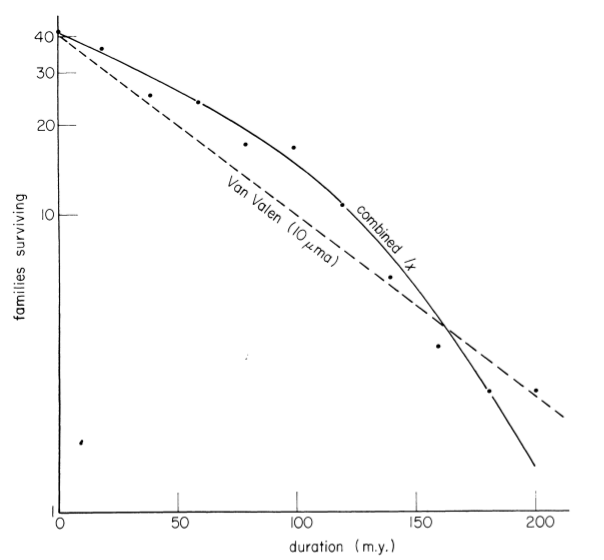
\includegraphics[height = 0.4\textheight, width = \textwidth, keepaspectratio = true]{figure/raup}

        \tiny{\attrib{Raup 1975 \textit{Paleobio.}}}

      \end{center}
    \end{column}
    \begin{column}{0.5\textwidth}
      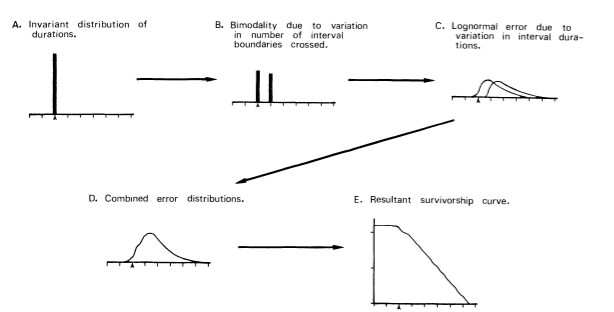
\includegraphics[height = 0.4\textheight, width = \textwidth, keepaspectratio = true]{figure/sepkoski}

      \tiny{\attrib{Sepkoski 1975 \textit{Paleobio.}}}

    \end{column}
  \end{columns}
\end{frame}

\begin{frame}
  \frametitle{Observe in simulation}

  Sampling: Poisson process (\(\phi\))

  Diversification: birth-death (\(\lambda, \mu\))

  \begin{enumerate}
    \item \(=\) birth, death; \(=\)preservation
    \item \(=\) birth, death; \(!=\)preservation
    \item \(!=\) birth, death; \(=\) preservation
    \item \(!=\) birth, death; \(!=\)preservation
  \end{enumerate}

\end{frame}

\begin{frame}
  \frametitle{The Elephant in the Range}
  \begin{center}
    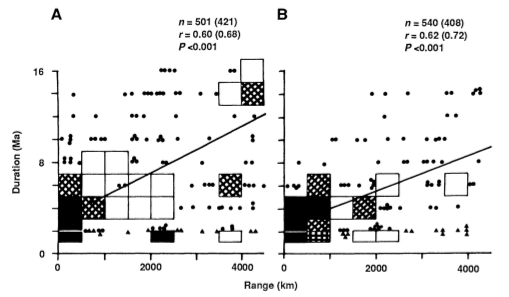
\includegraphics[height = 0.8\textheight, width = \textwidth,  keepaspectratio = true]{figure/range}

    \tiny{\attrib{Jablonski 1987 \textit{Science}}}
  \end{center}
\end{frame}

\begin{frame}
  \frametitle{Phylogeny and communities}

  \begin{center}
    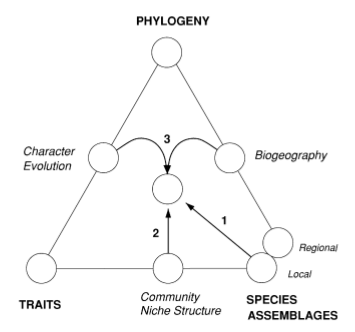
\includegraphics[height = 0.8\textheight, width = \textwidth,  keepaspectratio = true]{figure/webb}

    \tiny{\attrib{Webb \textit{et al.} 2002 \textit{Ann. Rev. Ecol. Syst.}}}
  \end{center}
\end{frame}

\begin{frame}
  \frametitle{(Informal) phylogeny}
  \begin{center}
    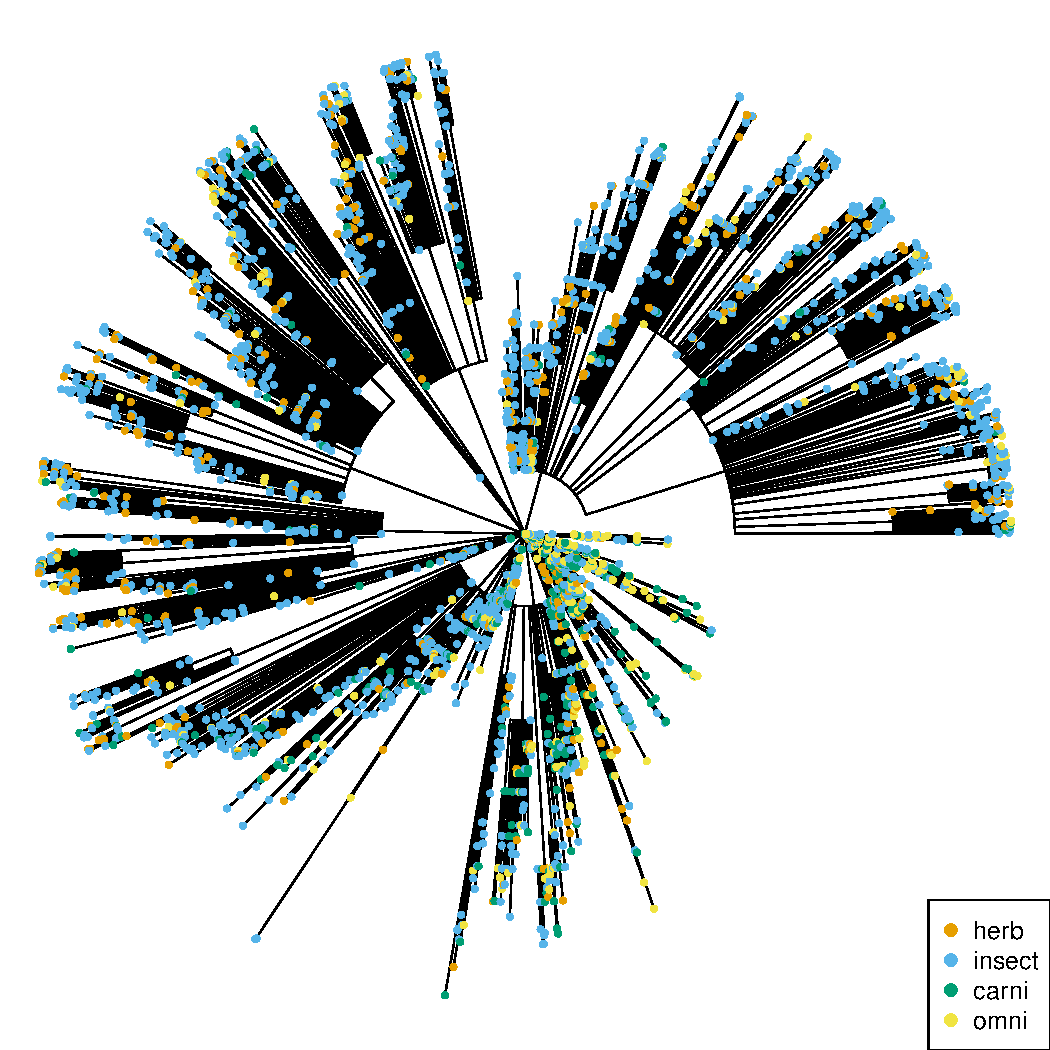
\includegraphics[height = 0.8\textheight, width = \textwidth,  keepaspectratio = true]{figure/na_phylo_diet}
  \end{center}
\end{frame}

\begin{frame}
  \frametitle{Compressing a network}

  \begin{block}{Map equation \tiny{\attrib{Rosvall and Bergstrom 2008 \textit{PNAS}}}}
    \begin{align*}
      L(\textbf{M}) &= q_{\curvearrowright}H(\mathcal{Q}) + \sum^{m}_{i = 1} p^{i}_{\circlearrowright}H(\mathcal{P}^{i})
    \end{align*}

    \begin{itemize}
      \item \(\textbf{M}\): module partion of \textit{n} nodes in \textit{m} partitions
      \item \(L(\textbf{M})\): theoretical minimum descriptive length of a single step
      \item \(q_{\curvearrowright}\): P(walk switches modules)
      \item \(H(\mathcal{Q})\): entropy of module codewords
      \item \(H(\mathcal{P}^{i})\): entropy within--module movements
      \item \(p^{i}_{\circlearrowright}\): fraction of within--module use in module \(i\)
    \end{itemize}
  \end{block}
\end{frame}

\begin{frame}
  \frametitle{Two-level compression}
  \begin{center}
    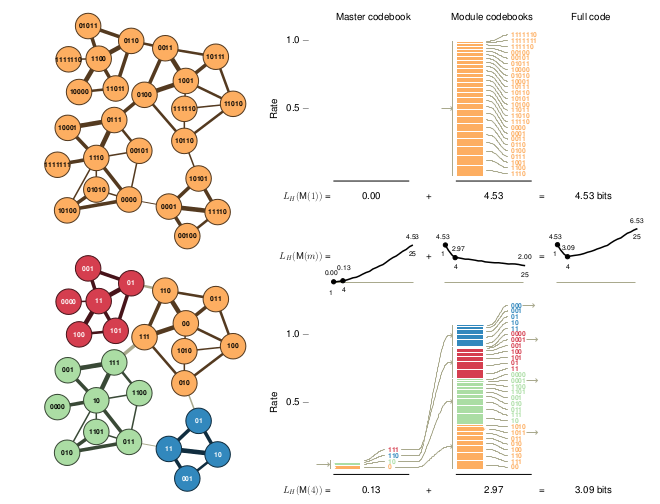
\includegraphics[height = 0.8\textheight, width = \textwidth,  keepaspectratio = true]{figure/code_expand}

    \tiny{\attrib{Rosvall and Bergstrom 2009 \textit{Euro. Phys. J. Spec. Topics.}}}
  \end{center}
\end{frame}


\end{document}
